\documentclass{article}
\usepackage{biblatex}
\addbibresource{literature.bib}

\usepackage{graphicx}
\usepackage[english]{babel}
\usepackage{caption}
\usepackage{csquotes}
\usepackage{xcolor}
\usepackage{subcaption}
\usepackage{authblk}
\usepackage{colortbl}
\usepackage{mathtools}
\usepackage{placeins}
\usepackage{graphicx}%
\usepackage{multirow}%
\usepackage{textcomp}%
\usepackage{booktabs}%e
\usepackage{listings}%
\usepackage{siunitx}
\usepackage[colorinlistoftodos]{todonotes}
\usepackage{hyperref}

%\setlength{\textwidth}{6.5in}
\usepackage[a4paper, total={6in, 8in}]{geometry}

\graphicspath{figures/}

\title{Advancing Reinforcement Learning Control: Continuous Scheme and Curriculum Learning for Mechanical Systems}

\author[1,2]{Oleg Rogov} 
\author[3]{Peter Manzl}
\author[3]{Johannes Gerstmayr}
\author[2]{Grzegorz Orzechowski}
\affil[1]{Savonia University of Applied Sciences}
\affil[2]{Lappeenranta-Lahti University of Technology LUT}
\affil[3]{University of Innsbruck}

% \date{January 2024}

\begin{document}

\maketitle

\listoftodos

\section{Introduction}

Multibody System Dynamics (MSD) is a field of study that concentrates on modeling, simulating, and analyzing the dynamics of systems composed of interconnected rigid and flexible bodies. It is a fundamental approach to understanding and predicting the dynamic behavior of complex mechanical systems through sophisticated mathematical models and computational algorithms. The essence of MSD lies in its capacity to accurately describe the motion, forces, and interactions among the components of a system and with the environment, considering both translational and rotational movements and the constraints that govern these movements~\cite{shabana2013dynMSD}. MSD is applicable across various engineering fields, from aerospace and automotive to biomechanics and robotics. This versatility underscores its capability to address the specific dynamics of different systems, enhancing its utility in diverse technological and scientific domains. Also, by accurately predicting system behavior, MSD supports the iterative design and optimization of mechanical systems. Engineers can use MSD to test and refine designs virtually, reducing the need for physical prototypes and accelerating the development process. One important characteristic of MSD is that the detailed models developed using this method make it an excellent foundation for implementing learning-based or model-based control strategies. These strategies, such as Reinforcement Learning (RL)~\cite{sutton_reinforcement_2018} and Model Predictive Control~\cite{schwenzer2021mpc}, can dynamically adapt to the system's behavior, leading to optimized performance even in complex and changing environments.

Reinforcement Learning, a primary control method used in our research, is a branch of Machine Learning (ML) where an agent learns to make decisions by taking actions in an environment to maximize the cumulative reward under acting according to a certain policy~\cite{sutton_reinforcement_2018}. In RL, rewards may not be immediate. An agent may need to perform a series of actions before receiving a reward, creating a delay between the initial action and the eventual reward. The learning process involves exploring various actions and states (exploration) and exploiting the knowledge gained to make better decisions (exploitation). The exploration and exploitation trade-off is one of the crucial concepts in reinforcement learning (RL), which emphasizes the need for a balance that results in efficient agent training. Achieving this balance is essential for the agent to learn effectively and optimize its performance over time. RL can be divided into two main types: model-free methods and model-based methods. The main difference between them is that in model-free methods the agent learns directly from interactions with the environment without trying to understand its dynamics, while in model-based methods the agent learns a model of the environment's dynamics and uses this model to plan and make decisions. Model-free methods are generally simpler and more robust in highly dynamic and complex environments, though they require more interactions for an agent to learn effectively. 
Additionally, RL can be further categorized into traditional Reinforcement Learning (RL) and Deep Reinforcement Learning (DRL). Traditional RL focuses on methods where the agent typically operates with simpler, lower-dimensional state spaces. These methods often rely on tabular representations or linear function approximations. DRL, however, specifically integrates deep neural networks to approximate value functions or policies, so that it can effectively handle high-dimensional state spaces and complex environments. This capability allows DRL to be applied to tasks such as playing video games, robotic control, and autonomous driving~\cite{roveda2020mbrl, mnih2013dqn, zhu2022inverted}. Examples of DRL methods are Advantage-Actor Critic (A2C), Proximal Policy Optimization (PPO) and Deep Q-Network (DQN). A2C is an advanced version of the actor-critic method that uses both policy (actor) and value (critic) functions, with the actor updating the policy based on feedback from the critic, enhancing stability and performance~\cite{mnih2016a2c}. PPO is a popular policy gradient method known for its robustness and simplicity, utilizing a clipped objective function to ensure stable learning~\cite{schulman2017ppo}. DQN combines Q-learning~\cite{sutton_reinforcement_2018} with deep neural networks to handle high-dimensional state spaces, approximating the Q-value function, which represents an expected cumulative reward an agent can achieve by taking a specific action in a given state and following the optimal policy, enabling it to learn effective policies in complex environments~\cite{mnih2013dqn}. 
In Reinforcement Learning, actions (control inputs) can be either discrete or continuous. Discrete actions are suitable for tasks where the set of possible actions is limited and distinct, such as choosing between different predefined options. Continuous actions, on the other hand, are used in scenarios where actions can take any value within a range, such as adjusting the speed of a car or the angle of a robotic arm. 
% RL is inspired by behavioral psychology and is gaining popularity in robotics, game playing, and optimization problems~\cite{roveda2020mbrl, mnih2013dqn, zhu2022inverted}.

The application of RL techniques in the context of MSD is still an emerging field, with limited research available. Current studies have primarily focused on traditional control methods, leaving significant potential for further exploration and development of RL-based approaches to enhance the adaptability and efficiency of MSD models. A noticeable study in this area is done by Kurinov et al.~\cite{kurinov2020autoexcavator}. Researchers have developed an autonomous excavator system utilizing RL as a control base integrated with MSD (detailed simulation with hydraulics and sensors). This study was focused on enabling the excavator to perform various tasks autonomously, including excavation and loading. The effectiveness of their approach was demonstrated in achieving autonomous operation with minimal collisions, showcasing the potential for automation in heavy machinery within the construction and mining industries.  
Additionally, Egli et al.~\cite{egli2022soil} explored the application of reinforcement learning (RL) for adaptive control in hydraulic excavators, aiming to enhance the automation of excavation tasks. Their study introduced a controller capable of adjusting to varying soil properties within a single excavation cycle. Utilizing an RL-based approach, they trained a control policy in simulation, integrating proprioceptive measurements to infer soil characteristics. This method demonstrated significant improvements in adaptability and efficiency compared to traditional excavation techniques. Notably, their controller could operate without explicit soil parameter inputs, relying instead on measurements from hydraulic pressure and kinematic sensors. The experiments conducted on a 12-ton excavator confirmed the controller's ability to maintain high performance across diverse soil conditions, emphasizing the feasibility of RL in real-world excavation scenarios.
Furthermore, Osa and Aizawa~\cite{osa2022deep} investigated deep reinforcement learning with adversarial training for automated excavation. They proposed a novel regularization method that employs virtual adversarial samples to mitigate the overestimation of Q-values in a Q-learning algorithm. Their approach, which integrates depth images for excavation planning, demonstrated superior sample efficiency and robustness in policy learning compared to traditional actor-critic methods~\cite{sutton_reinforcement_2018}. This research highlights the importance of incorporating visual information and advanced regularization techniques to enhance the reliability and effectiveness of RL-based systems.

While RL has shown considerable promise as a control method for complex dynamic systems, it is not without its limitations. One of the primary challenges of RL is its high demand for extensive interactions with the environment to learn effective policies, which can result in long training times and high computational costs. Additionally, RL algorithms often struggle with the exploration-exploitation trade-off, especially in high-dimensional state spaces and non-linear dynamics typical of MSD. These factors can make RL less efficient and robust when applied directly to complex mechanical systems~\cite{dulac2019challenges}.
This is where Curriculum Learning (CL) can provide substantial benefits. CL is about structuring training content and learning experiences in a way that mirrors the progression from simple to complex, akin to how a curriculum in educational settings is designed~\cite{bengio2009cl}. This method may not only accelerate the learning process but also enhance the robustness and adaptability of the control strategies.
Research by Hacohen et al.~\cite{hacohen2019clnetworks} delves into the effectiveness of CL in the training of deep neural networks, with a focus on how CL can significantly impact the efficiency of the learning process. Experiments to analyze the impact of curriculum-based learning on the training efficiency of deep neural networks were conducted and the curriculum was structured around a series of tasks, each representing a different level of difficulty, designed to challenge the neural network progressively. This method allowed for the examination of how neural networks adapt their learning strategies in response to escalating task complexity. This work suggests that by implementing a curriculum-based approach deep RL algorithms can develop more robust and effective strategies.


The work by Narvekar et al.~\cite{narvekar2020survey} is particularly instructive for our research as it provides a taxonomy of CL methodologies that can be directly applied to the RL challenges we could face in tandem with MSD. They categorize CL strategies into three main approaches: task sequencing, transfer learning, and multi-task learning. Task sequencing involves arranging learning tasks in a meaningful order to gradually increase complexity, thereby enhancing the learning efficiency and robustness of RL agents. Transfer learning focuses on leveraging knowledge gained from previous tasks to improve performance on new, related tasks. Multi-task learning allows simultaneous training on multiple tasks to share knowledge and improve overall learning efficiency. By structuring the learning experiences from simple to complex tasks, we can systematically improve the RL agent's ability to handle the difficulties of mechanical systems in MSD. In our research an implementation of transfer learning can be useful, since we can start training inverted pendulum on a cart as a simple one-link system and then increase the complexity of it by adding more links. This systematic enhancement of learning experiences can mitigate some of the efficiency and robustness issues traditionally associated with RL in dynamic, high-dimensional environments.

Furthermore, Weinshall's work~\cite{weinshall2018cltransfer} have delved into the integration of TL within CL, highlighting how accumulated knowledge can significantly boost performance in more complex systems. Their work demonstrates that using a pre-trained neural network on a different task to guide the curriculum can approximate an ideal learning sequence, leading to faster convergence and improved generalization. 

The study written by Gupta et al.~\cite{gupta2021rlcapabilities} investigates how integrating CL can enhance RL for continuous control tasks, which are highly relevant to MSD. Their research focuses on tasks such as robotic arm manipulation and locomotion, demonstrating that various CL strategies, like progressive task sequencing and parameter adaptation, significantly improve learning efficiency and performance. 

A paper by Bhati et al.~\cite{bhati2023clmulti} demonstrates the effectiveness of CL in a multi-agent RL environment. A sequential task structure was implemented where each task increased in complexity and inter-agent dependency. This approach was designed to incrementally develop and refine the cooperative strategies of individual agents within a simulated multi-agent environment, allowing researchers to observe how agents adapted and optimized their performance in progressively challenging scenarios. This finding is crucial for tasks where teamwork among agents is a key factor. 

The perspectives of using Curriculum Reinforcement Learning (CRL) in mechanical system dynamics (MSD) are promising. CRL, which integrates Curriculum Learning (CL) with Reinforcement Learning (RL), offers a structured approach to tackle the complexities of MSD by gradually increasing the difficulty of control tasks. This methodology enhances learning efficiency and improves the adaptability and robustness of RL agents in managing dynamic mechanical systems. Additionally, continuous RL plays a crucial role in this context. Unlike discrete RL, continuous RL allows for more precise and smooth control by operating within a continuous action space. This capability is an important point for the system of our study, the inverted multi-link pendulum on a cart, where maintaining stability and controlling the pendulum’s oscillations demand precise and continuous adjustments to manage the complex, nonlinear dynamics of the system effectively. In our prior work by Manzl et al.~\cite{manzl2023relrl}, we evaluated RL algorithms for controlling mechanical systems using discrete control methods, effectively stabilizing single to triple link inverted pendulum systems. The RL approach demonstrated adaptability and effectiveness in managing the dynamics and complexities of these models. Our current study extends this work by applying a novel continuous control method combined with CL technique. Using the same multi-link inverted pendulum on a cart system, we can clearly demonstrate the improvements afforded by these advanced methods. By switching from discrete to continuous action space, we enable smoother and more precise adjustments in system behavior with the faster training time, which are critical when managing the complex dynamics of multibody systems. Moreover, integrating CL accelerates the training process more, allowing RL agents to quickly adapt to increasingly complex tasks. This dual approach not only streamlines control operations but also significantly enhances learning efficiency. Our empirical evidence demonstrates the effectiveness of these strategies in a controlled mechanical environment, highlighting their practical implications. This research paves the way for developing more advanced, autonomous control systems that could transform interactions with mechanical systems across various industries.
\section{Methods}

\subsection{Mechanical model}

The system under investigation is a multi-link inverted pendulum on a cart. This setup, known for its inherent instability and dynamic nature, is a cornerstone in control theory~\cite{Fantoni2001Nonlinear}. The cart, serving as the base platform for the pendulum links, is limited to linear motion along a horizontal track, simplifying the translational dynamics to one-dimensional motion along the x-axis. The cart's movement is controlled by an externally applied force $F$, which is crucial for the system's stabilization. The magnitude and direction of this force significantly impact the system's dynamics, providing a means to counteract the gravitational torque imposed by the pendulum links. The details of the system modelling are described in~\cite{manzl2023relrl}.

\begin{figure}[h]
\centering
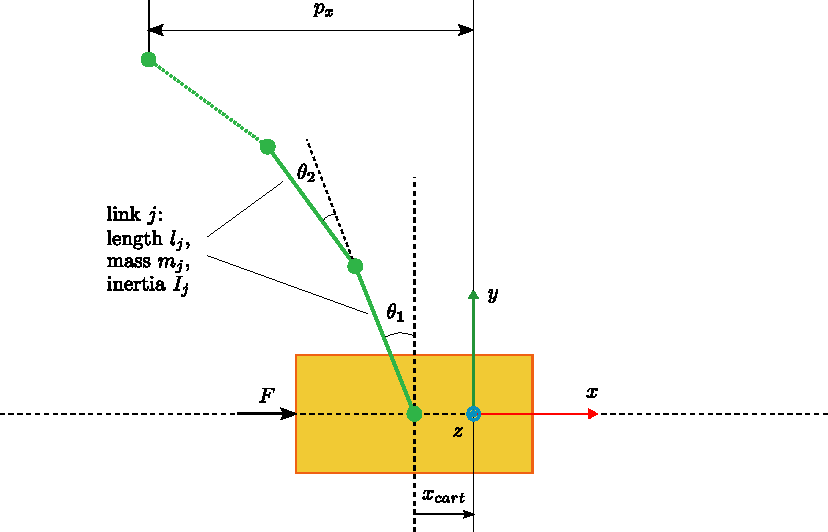
\includegraphics[width=10cm]{Figures/cart_pole_model.pdf}
\caption{$N$-link inverted pendulum on a cart. Minimal coordinates formulation $\mathbf{q} = \mathbf{s} =  [x_{\text{cart}}, \theta_1, \ldots, \theta_N]$ are used to model the system. Each link consists of length $l_j$, mass $m_j$, moment of inertia $I_j$. The cart is a rigid body with mass $m_{cart}$.}
\label{fig: n-pendulum on a cart}
\end{figure}

Attached to the cart is a series of n rigid links, each connected end-to-end by revolute joints. These joints allow for free rotational movement in the vertical plane, and each link 
$j$ is characterized by mass $m_j$, length $l_j$ and inertia $I_j$.
This model, with its high degree of control difficulty and relevance to real-world applications, provides a valuable platform for testing sophisticated control algorithms, including those based on Reinforcement Learning.

\subsection{Reinforcement Learning with continuous action space}
Reinforcement Learning is a branch of machine learning where an agent learns optimal behavior through systematic interaction with a dynamic environment, aiming to maximize cumulative rewards. This learning paradigm is distinct from supervised learning; in RL, the agent is not explicitly instructed which actions to take. Instead, it must explore and discover which actions yield the highest rewards by trial and error, a process often facilitated by a policy—a decision-making function that maps states of the environment to actions to be taken in those states~\cite{sutton_reinforcement_2018}.

In our research, RL is employed to train agents to manage the dynamics of a multi-link inverted pendulum on a cart, a challenging control problem that requires maintaining precise dynamic stability throughout the process. The reward function in RL plays a crucial role as it guides the learning process. For instance, a reward function can be designed to penalize the agent for excessive movement away from a target state or for using too much energy, while rewarding closer approximations of the desired state, such as maintaining the pendulum in an upright position. We use the reward function, which has shown one of the best performances from our previous study
\begin{equation}
r = 1 - w_p \frac{\left|p_x\right|}{\chi_\mathrm{cart}} - (1-w_p) \frac{\sum_{j=1}^\mathrm{N} \left|\theta_j\right|}{\mathrm{N} \chi_{\theta}} 
\label{eq:reward}
\end{equation}
It combines a tip position with the sum of pendulum link angles $\sum_{j=1}^{N} \left|\theta_j\right|$, weighted by a factor $w_p$. $\chi_\mathrm{cart}$ and $\chi_{\theta}$ are predefined, constant position and angle thresholds, which differ from 1-link to more link systems. $\mathrm{N}$ is the number of the links.

In RL, the choice between discrete and continuous action space might significantly affect the performance of learning algorithms. Discrete action space, used in our previous study, limits the agent’s actions to a finite set of possibilities: it either applies a negative or a positive force of the same magnitude to regulate the behavior of the system. In a continuous action space the agent is provided with an interval of the control force
\begin{equation}
F = [-f_\mathrm{cart}, +f_\mathrm{cart}]
\label{eq:force}
\end{equation}
From this interval in Eq.~\eqref{eq:force} the agent is free to choose any suitable control force as an action for learning the stabilization task. Since it provides more possible actions then the discrete action space, it emerges in a faster training of an agent and achieves a more smooth and robust control task execution.  
% NOTE: 1) continue with - adding a final punchline to this section
% While simpler to implement, this can restrict the agent's ability to finely tune its responses to the environment's demands.

\subsection{Model evaluation} \label{Model evaluation}

\todo[inline, color=green, size=\small]{When you answer the todo, please add an option \texttt{disable} to it (as in the one below) so that it is not shown in text, but I know what was to be done. Thanks.}

\todo[inline, disable]{Due to \texttt{disable} option, it does not show in text.}

\todo[inline]{Write a single paragraph explaining the model evaluation in simple words.}

For the model evaluation we use the same specifications as in our previous research of Manzl et. al.~\cite{manzl2023relrl}. The performance of the agent is periodically evaluated based on the mean reward exceeding a defined threshold \( \lambda_r \) and the loss being below a threshold \( \lambda_l \)\todo{This statement is inaccurate. Is it really the base for evaluation?}. During each evaluation, the agent undergoes \( n_{\text{test}} \) tests in an environment simulated for \( n_{\text{eval}} \) time steps, ensuring \( n_{\text{eval}} > n_{\text{learn}} \)\todo{Write what does this inequality means}. For instance, with a time step \( h = 0.02 \) s, \( n_{\text{eval}} = 5000 \) corresponds to a 100 s test duration. During the tests, the agent's initial states are perturbed within a range of \( \pm x_{\text{init}} \), and the maximum norm of the state vector is used to compute the test error \( e_{\text{test},i} = \|\mathbf{s}_i\|_{\infty} \) at each time step \( t_i \). The total test error \( e_{\text{test}} \) is defined as the maximum error encountered in the final quarter of the evaluation period:
\begin{equation}
	e_{\text{test}} = \max(e_{\text{test},i}) \quad \forall \, i \geq \frac{3}{4}n_{\text{eval}}.
\end{equation}
The training is deemed complete when \( e_{\text{test}} \) falls below a pre-determined threshold \( \chi_{\text{test}} \) for all tests, providing a criterion for potential early stopping. To assess model robustness, several agents are trained and evaluated, with their performances depicted as envelopes formed by the best, worst, and mean error metrics across time steps. Notably, early evaluation results (within the first 50,000 steps\todo[]{Does the same value is valid for each $n$-pendulum?}) may be unreliable due to insufficient model development, necessitating the use of linear interpolation for clearer data interpretation.

\subsection{Performance evaluation of PPO with continuous action space} \label{subsec: Performance Evaluation of PPO with Discrete and Continuous Action Spaces}

For the evaluation of an action space benefits\todo[]{What is the 'evaluation of an action space benefits'. Make it clearer.} in our study we use the PPO RL-algorithm. PPO algorithm itself aims to improve policy gradient methods\todo[]{This note is unclear without any reference to what 'policy gradient methods' are any why they need improvements. It is neede?} by optimizing a surrogate objective function\todo[]{This is even more confusing. Rewrite.} while ensuring that updates to the policy do not deviate too far from the previous policy. It accomplishes this by using a clipped objective function that limits the size of policy updates, thereby stabilizing training and improving performance~\cite{schulman2017ppo}. The evaluation is conducted on an N-link inverted pendulum system, specifically analyzing the performance with 1-link, 2-link, and 3-link systems. The analysis explores two different action spaces and their impact on the agent's ability to stabilize the pendulum in the upward-facing equilibrium. 
For all systems, we focus on the task of balancing the inverted pendulum in the unstable upward-facing equilibrium. The challenge increases with the number of links, as each additional link contributes to the overall instability of the system. The single pendulum is a well-known benchmark for RL methods, and this evaluation extends to more complex systems with additional links.
The experiments are conducted using Exudyn Version 1.8.52 and stable-baselines3 Version 1.8.0. Each experiment is repeated 10 times with different random seeds to account for variations in initialization. The PPO algorithm is implemented\todo[]{Used? I do not think we have implemented it.} with standard parameters, except where adjustments are made for the specific requirements of the environment.

Table~\ref{tab:hyperparameters} summarizes the hyperparameters used in the experiments, and Table~\ref{tab:env_params} outlines the environment, reward, and training parameters for the different link configurations. Notably, the cart force is now continuous and is presented as an interval, ranging from \([-12, 12]\) N for the 1-link system, and similarly for the 2-link and 3-link systems\todo[]{Show numbers for all cases or none of them.}.

\begin{table}[h]
	\centering
	\caption{The hyperparameters used for the PPO method in the experiments. The physical parameters are provided in Table~\ref{tab:env_params}.}
	\label{tab:hyperparameters}
	\begin{tabular}{ll|ll}
		\toprule
		\textbf{Parameter}       & \textbf{Value} & \textbf{Parameter}       & \textbf{Value} \\ \midrule
		Reward function          & $r$, Eq.~\ref{eq:reward},  & Reward threshold         & $\lambda_r = 0.9$ \\ 
		Step size                & 20 ms           & Loss threshold           & $\lambda_l = 0.01$ \\ 
		Evaluation length        & 5000 steps $\Rightarrow$ 100 s & PPO: $n_{\text{steps}}$       & $n_{\text{episode,max}}$ \\ 
		Learning rate      & $5 \cdot 10^{-4}$ & & \\ \bottomrule
	\end{tabular}
\end{table}

\begin{table}[h]
	\centering
	\caption{Environmental, reward, and training parameters for the environments with link numbers 1 to 3.}
	\label{tab:env_params}
	\begin{tabular}{l l c c c}
		\toprule
		\textbf{Name} & \textbf{Parameter} & \textbf{1 link} & \textbf{2 link} & \textbf{3 link} \\ \midrule
		Cart force              & $f_{\text{cart}}$ in N         & \([-12, 12]\)   & \([-40, 40]\)   & \([-60, 60]\)  \\ 
		Threshold cart position & $\chi_x$ in m                 & 1.2  & 3.6  & 5.4 \\ 
		Threshold link angle    & $\chi_\varphi$ in rad         & $\frac{\pi}{20}$ & $\frac{\pi}{10}$ & $\frac{3\pi}{20}$ \\
		For $\theta_1$ to $\theta_N$ \todo[inline, size=\tiny, inlinewidth=3cm]{Is this needed here? Confusing.} & & & & \\
		Max test error          & $e_{\text{test}}$             & 0.2  & 0.5  & 0.75 \\ 
		Reward position factor  & $w_p$                         & 0.5  & 0.5  & 0.8 to 1 \\ 
		Required training steps & $n_{\text{learn}}$            & $80 \cdot 10^3$ & $150 \cdot 10^3$ & $350 \cdot 10^3$ \\ 
		Max episode length      & $n_{\text{episode,max}}$      & 1280 & 1536 & 2048 \\ 
		Tests per evaluation    & $n_{\text{test}}$             & 50   & 50   & 100 \\ 
		\bottomrule
	\end{tabular}
\end{table}

The continuous action space, particularly in the control of the cart force, provides more nuanced control via the specified interval of the force, which is expected to influence the stabilization process, especially in the more complex multi-link systems.

\subsection{Curriculum learning implementation} \label{subsec: Curriculum learning implementation}
Our approach to Curriculum Learning in the domain of MSD is rooted in the incremental introduction of complexity to the learning environment of the RL agent, which, according to the taxonomy provided in~\cite{narvekar2020survey}, is based on Transfer Learning.
In our study, the concept of CL is physically represented through the introduction of spring-damper elements, which play a crucial role in regulating the dynamic behavior of the system under study\todo[]{The second part of this sentence is unclear. What plays a crucial role and what does 'regulating the dynamic behavior' means in our context?}. These spring-damper elements are strategically positioned between different components of the system to modulate the interactions and stability during the learning process. A schematic view of this physical representation is illustrated in Figure~\ref{fig: cl mechanical implementation}. Here, we utilize two types of spring-damper systems: a translational spring-damper and a rotational spring-damper. The translational spring-damper is connected between the cart body and the ground. Its primary function is to restrict the translational movement of the cart along the x-axis. By controlling this movement, the translational spring-damper indirectly adjusts the speed of the pendulum system, ensuring stability during the initial learning phases\todo[]{Make this statement more straighforward and clear.}. This stability is vital for the agent to safely explore the system dynamics without being overwhelmed by excessive movement. The rotational spring-damper systems are attached to the revolute joints, regulating the angular displacement of the pendulum. These systems provide resistance to angular changes, thus preventing abrupt rotational movements that could destabilize the learning process. By controlling the angular behavior, the rotational spring-dampers ensure that the pendulum remains within a manageable range of motion during the early stages of learning.

\begin{figure}[h]
	\centering
	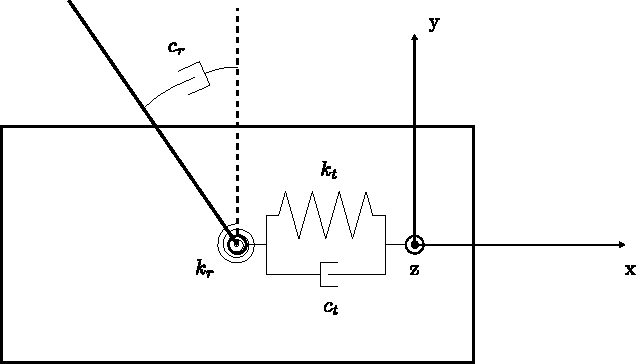
\includegraphics[width=10cm]{Figures/cl_mech_implementation_v1.pdf}
	\caption{Scheme of the system with translational and rotational spring-dampers. \todo[inline]{Make it consistent with Figure 1.}}
	\label{fig: cl mechanical implementation}
\end{figure}

These mechanical components provide physical constraints\todo[]{Totally inaccurate. What is the constraint in multibody dynamics?} that simplify the learning environment, enabling the agent to gradually adapt to the complex dynamics of the system. \hl{As the training progresses, the influence of these spring-damper systems is systematically reduced, allowing the agent to take more control over the system. In the later stages of training, the spring-dampers' effects are diminished, either by reducing their stiffness and damping coefficients or by removing them entirely, thus transferring full control to the learning agent. This transition is crucial for ensuring that the agent is not overly reliant on the physical constraints and is capable of managing the system dynamics independently.}\todo[]{Rewrite the selected part. Make it shorter, easier to read.}
Following this physical setup\todo[]{What physical setup you are referring here?}, We have four parameters in our CL-scheme\todo[]{Description of those parameters is unclear as the setup is not defined. You must include decay functions and show how they are parametrized.} and their roles are explained in the Table~\ref{table: decay types}. 

\begin{table}[h]
	\caption{Decay types and their descriptions}
	\centering
	\begin{tabular}{l|p{0.7\textwidth}}
		\toprule
		\makecell{\textbf{Curriculum}\\ \textbf{Learning}\\ \textbf{parameters}} & \textbf{Description} \\ \midrule
		Control values & control parameters representing spring-damper values, which influence the restriction of the system behavior\\ \hline 
		Decay steps & time steps when the transition to another set of control values occurs\\ \hline 
		Decay function & describes the law on how the control values will be changed\\ \hline
		Decay factor & sets the speed of decay function\\ 
		\bottomrule
	\end{tabular}
	\label{table: decay types}
\end{table}

Our approach involves predefined decay functions that dictate the rate and pattern of assistance withdrawal, ensuring a smooth transition of control from the spring-damper systems to the agent. The comparison of decay functions behavior, which are used in our study, is showed at the Figure~\ref{fig: decay functions}.\todo[]{Those functions require more detailed description.}

\begin{figure}[ht]
	\centering
	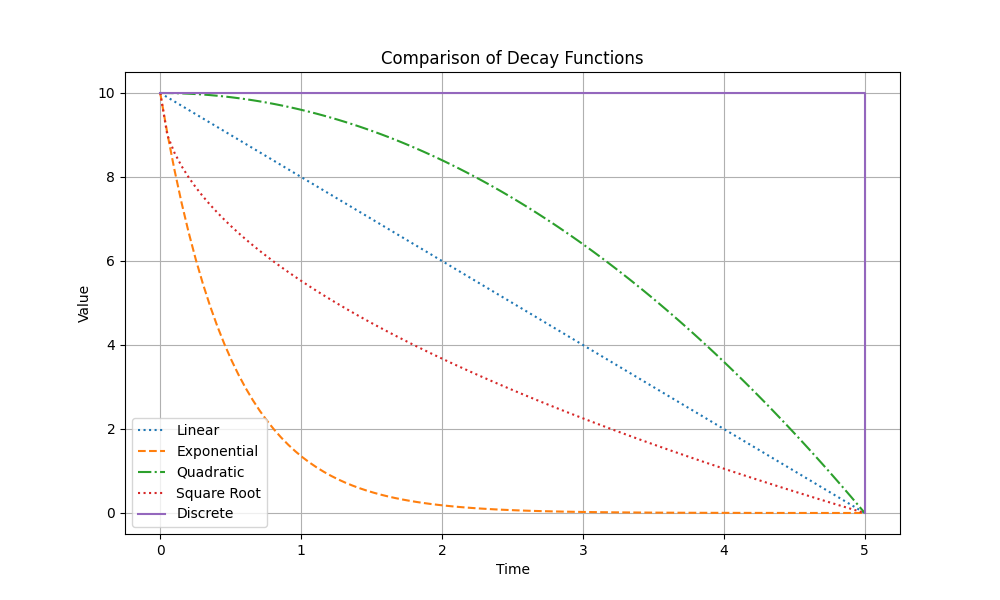
\includegraphics[width=13cm]{Figures/CL_decay_types_comparison.png}
	\caption{5 decay functions comparison for a given set of control values [10, 0]. At the decay step equal to 5 all the functions take the next control value of 0.}
	\label{fig: decay functions}
\end{figure}

\section{Results}

In this section we examine the performance of the state-of-the-art RL algorithm PPO for a discrete and continuous action spaces and show how can CL influence the overall learning task. Most of the results for comparison of the discrete action space are taken from our previous paper~\cite{manzl2023relrl}. First subsection presents the results achieved while comparing the trained agent with the same initial parameters using continuous and discrete control schemes. Second subsection describes the work of an agent in a modified environment, where the physical parameters of the system are changed. In the last subsection we present the role of CL in the enhancement of the overall RL agent training. 
% put the plot from extended abstract
% sectionalize this part: 
% 1) basic comparison of continuous with discrete for: SP, DP(the stability zones are not ready yet), TP(?, not on-going) - stability zones + training time (continuous and discrete plots for 100k timesteps alike)
% 2) physical values change influence
% 3) CL enhancement (how does it influence RL?) results - what could be shown there? Training time (from the extended abstract at least): for SP, DP (not prepared), TP (not on-going) and possibly QP (in plans)
%%%% MUST ASK GRZEGORZ ABOUT THE SMALL CODE PART TO RUN THE TP WITHOUT ISSUES

\subsection{RL with continuous action space} \label{subsec: RL with continuous action space}

\todo[inline=true]{You must introduce the details of the system first. It means, description of the system and numbers provided. If the system is already described, like here, you must reference and provide missing information. Same applies to algorithm, reward (what are thresholds), number of runs, etc.}

\todo[inline=true, color=cyan]{Before you will show the stability zones, you must provide a plots about the training itself. So the reward plots as a function of epochs. It is important to point out that the training has converge and to know what are the parameteres of training algorithm as well. Stability zones cames later. As such, change the order of the plots. Remember that firstly, you are explaining in details what you are showing. Next, you are providing the interpretation of results.}

For a better evaluation of the continuous control scheme in comparison to the discrete one, we have created a stability zone\todo{You must explain what stability zone is.}, the development of which is described in our work of Manzl et al.~\cite{manzl2023relrl}. From an engineering standpoint, not only are the randomized tests used for evaluation important, but it is also crucial to identify an area where the agent successfully performs the stabilization task for practical, real-world applications.\todo{Put this sentence later, after you present the results and explain their meaning. And discuss how the results you are showing agree with your statement.} The stability zone is shown in Figure~\ref{fig: continuous vs discrete}. A heatmap displays test results across a grid of parameters, plotting the link's angle on the X-axis and angular velocity on the Y-axis. The continuous control scheme, which replaces the earlier discrete scheme, demonstrates a broader area of optimal performance and smoother transitions at boundary conditions, suggesting improved control capabilities.\todo{Add more details based on the Figure. You can analyze each of the subfigures in details. Explain what each subfigure shows. You should not add a big Figure and summarize it by saying \textit{it works better}.}

\begin{figure}[h!]
	\centering
	\begin{subfigure}[t]{0.48\textwidth}
		\centering
		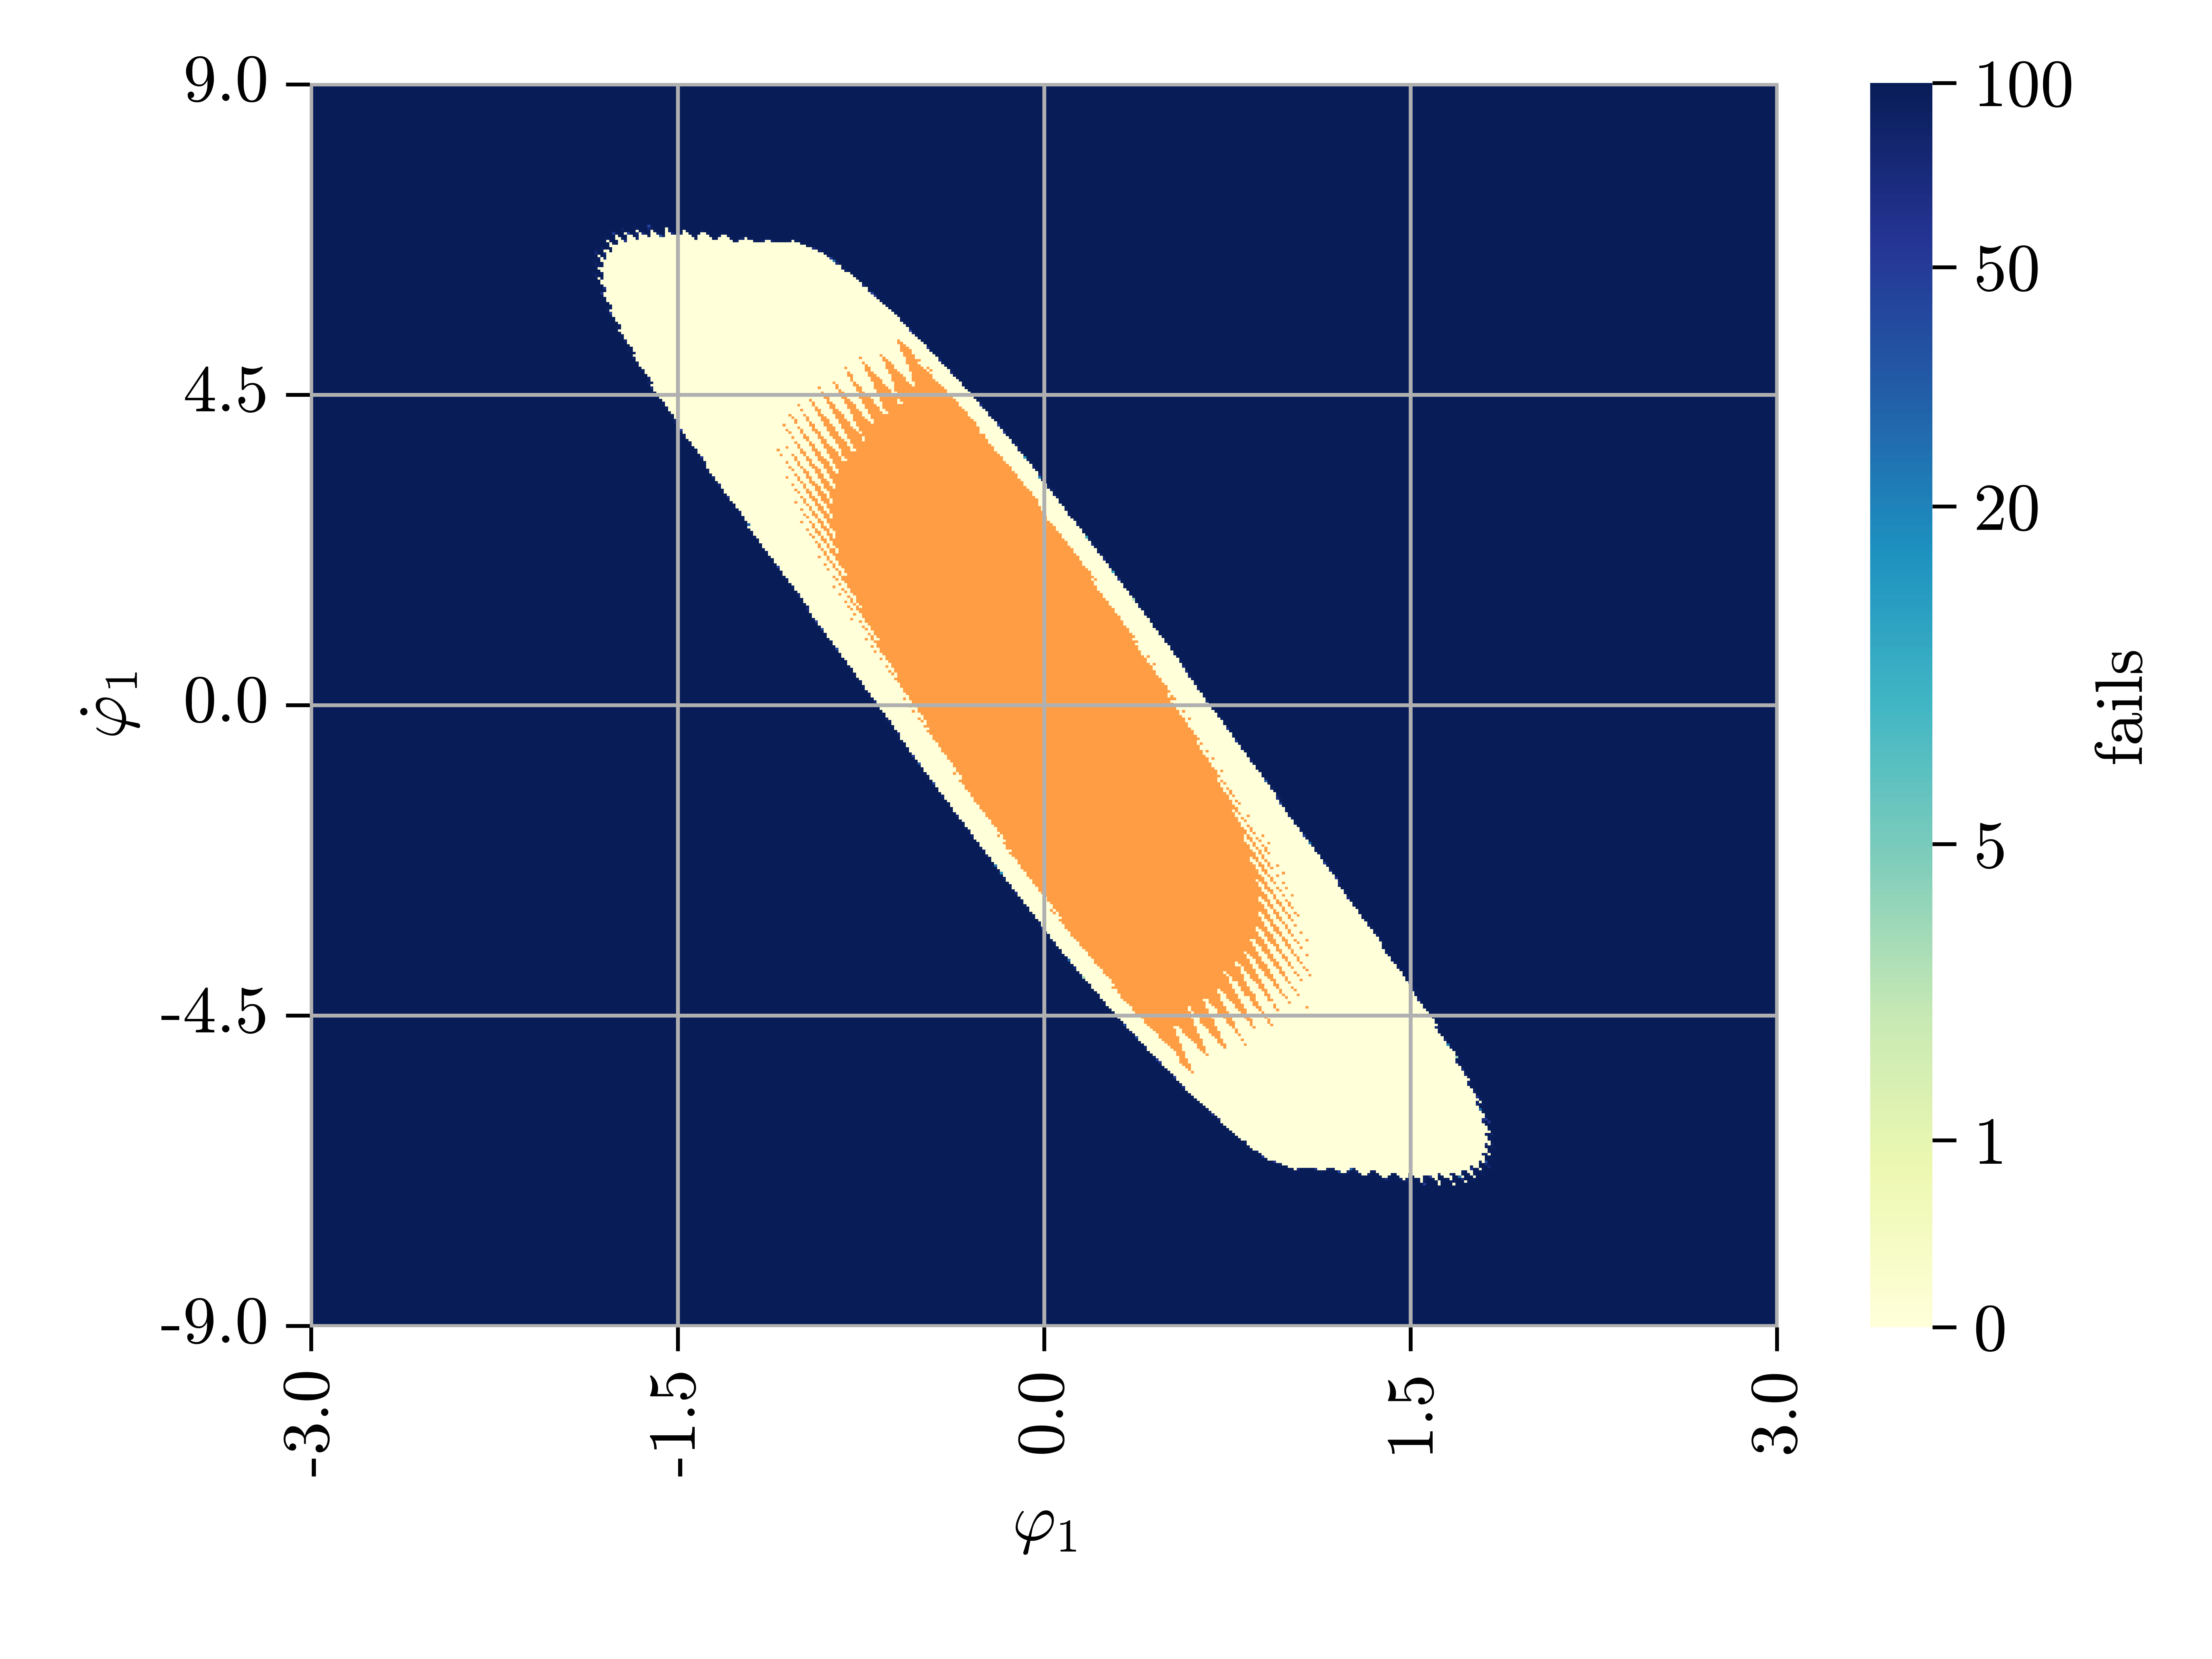
\includegraphics[width=\textwidth]{Figures/SP_continuous_vs_discrete_phi1phi1dot.png}
		\label{fig: sp - continuous vs discrete}
		\caption{}
	\end{subfigure}
	\hfill
	\begin{subfigure}[t]{0.48\textwidth}
		\centering
		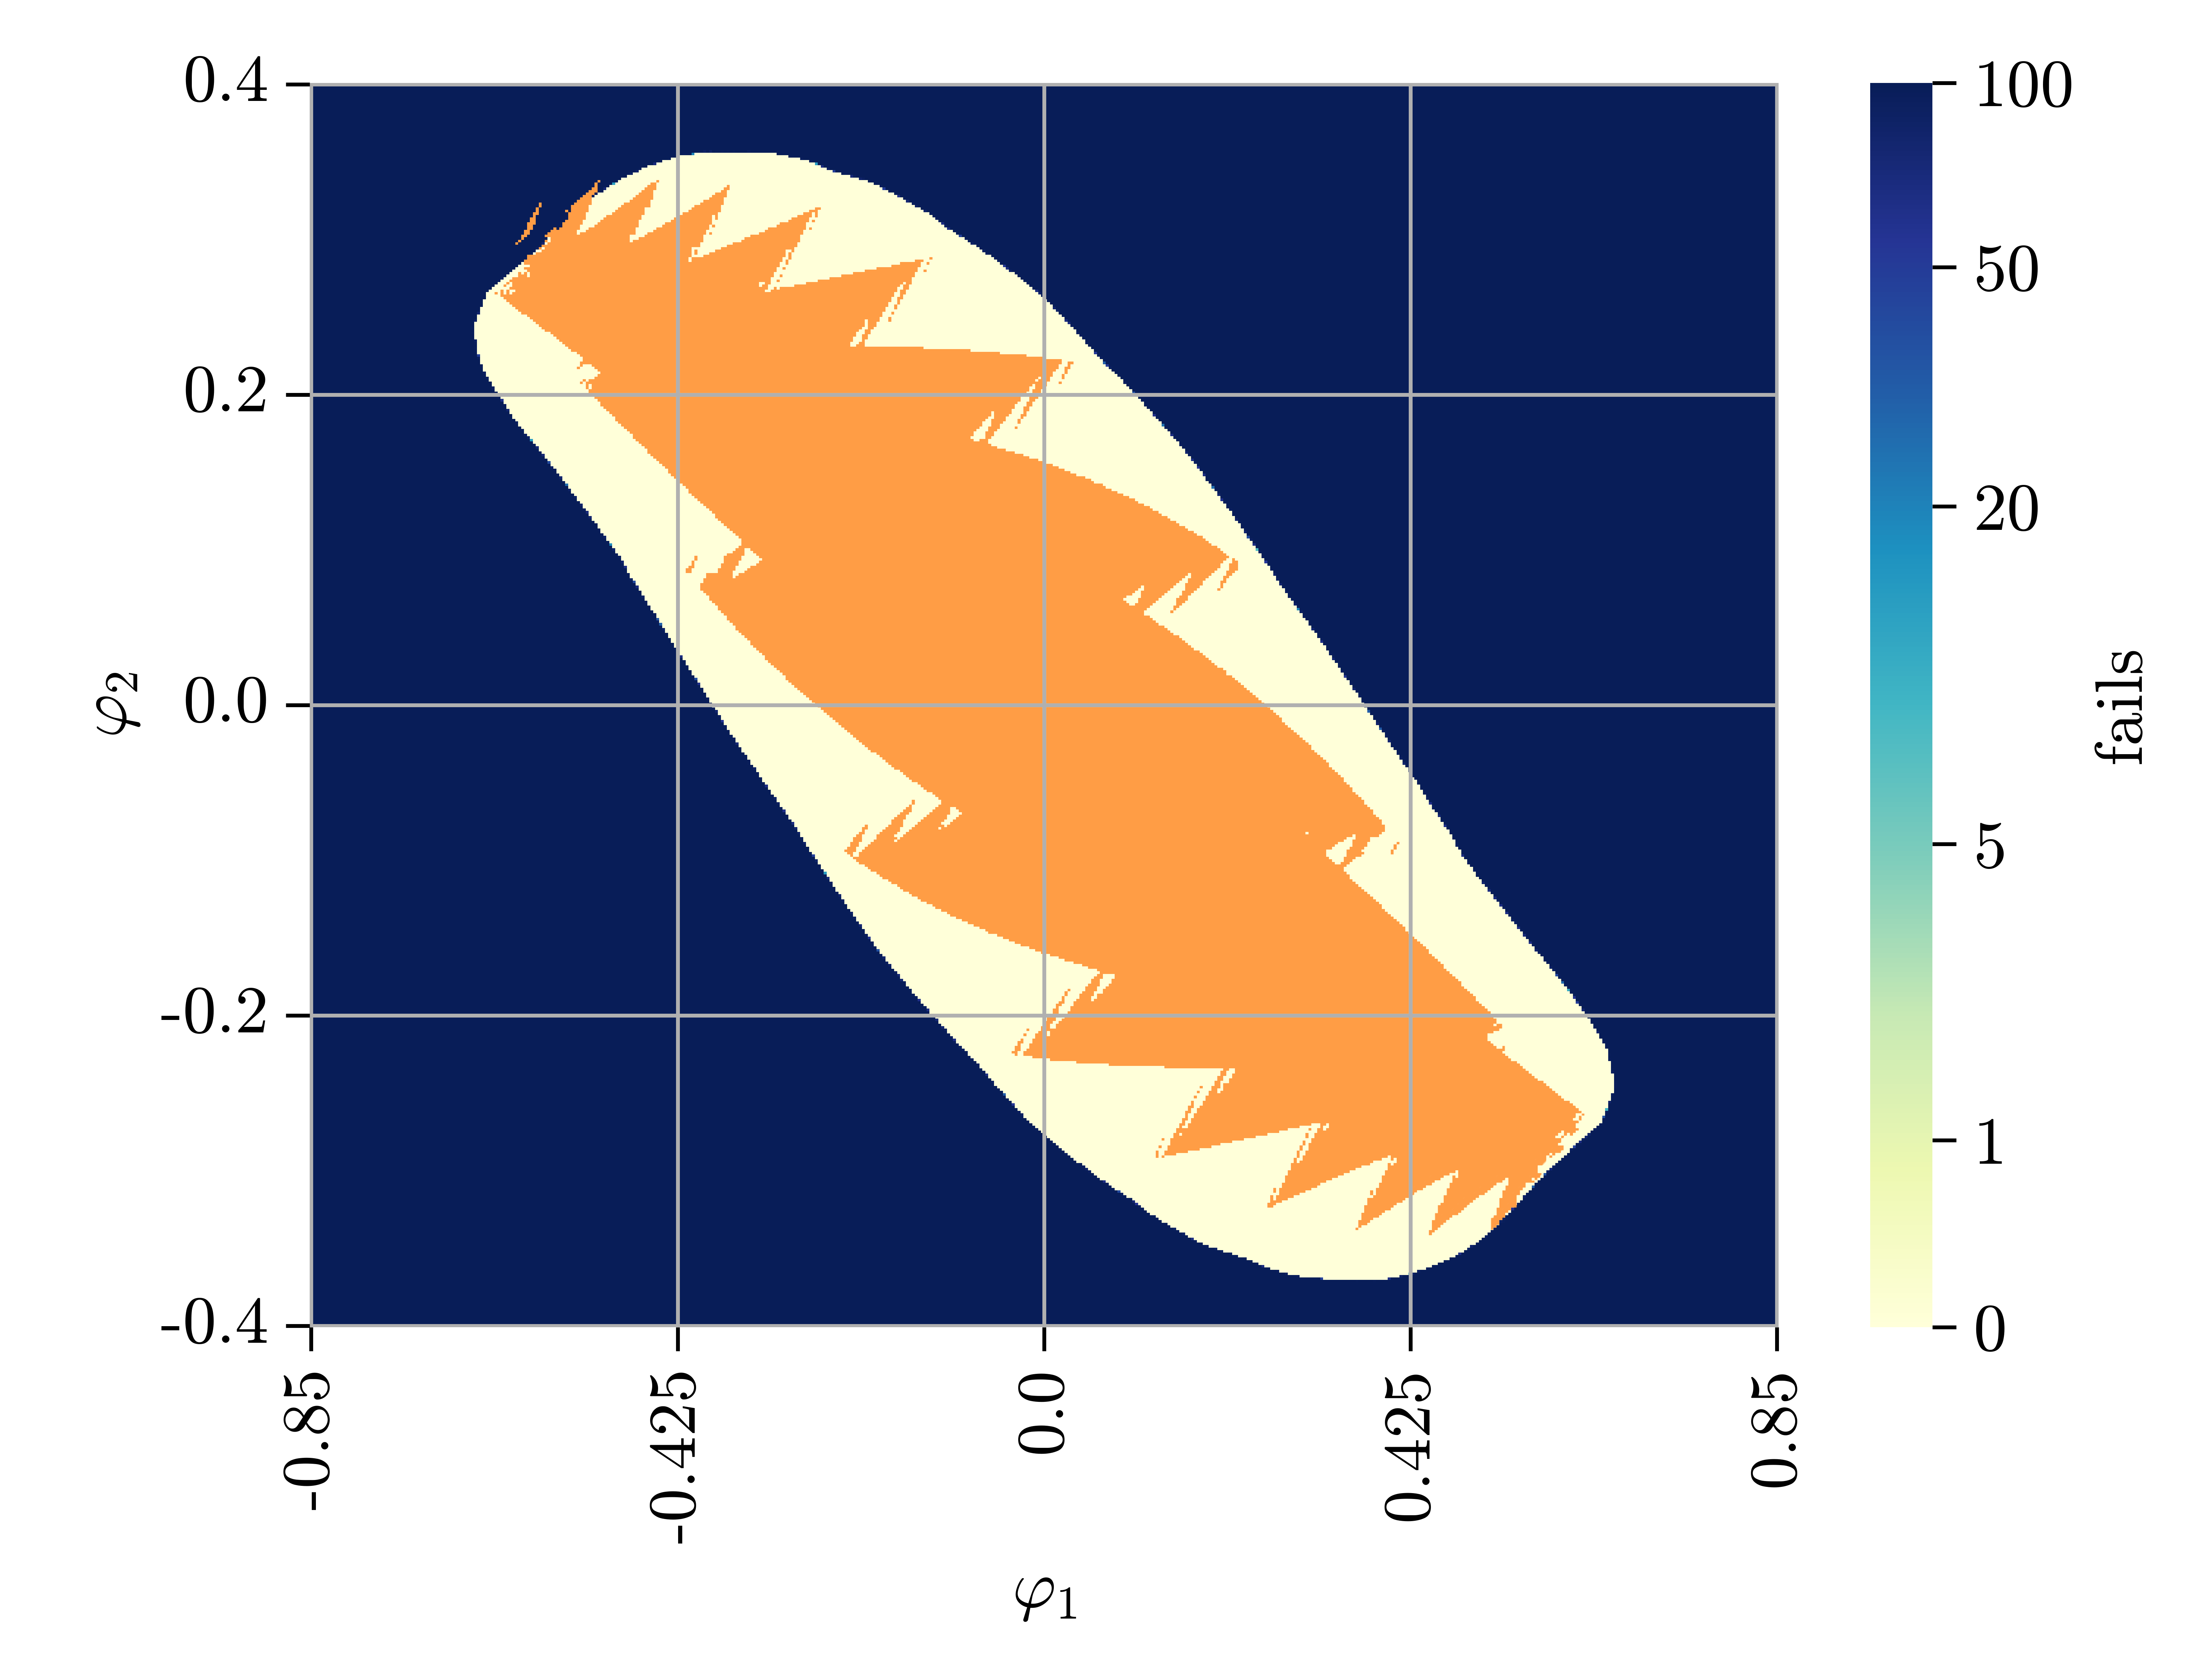
\includegraphics[width=\textwidth]{Figures/DP_continuous_vs_discrete_phi1phi2.png}
		\label{fig: dp - continuous vs discrete}
		\caption{}
	\end{subfigure}
	
	\vspace{0.2cm}
	
	\begin{subfigure}[t]{0.48\textwidth}
		\centering
		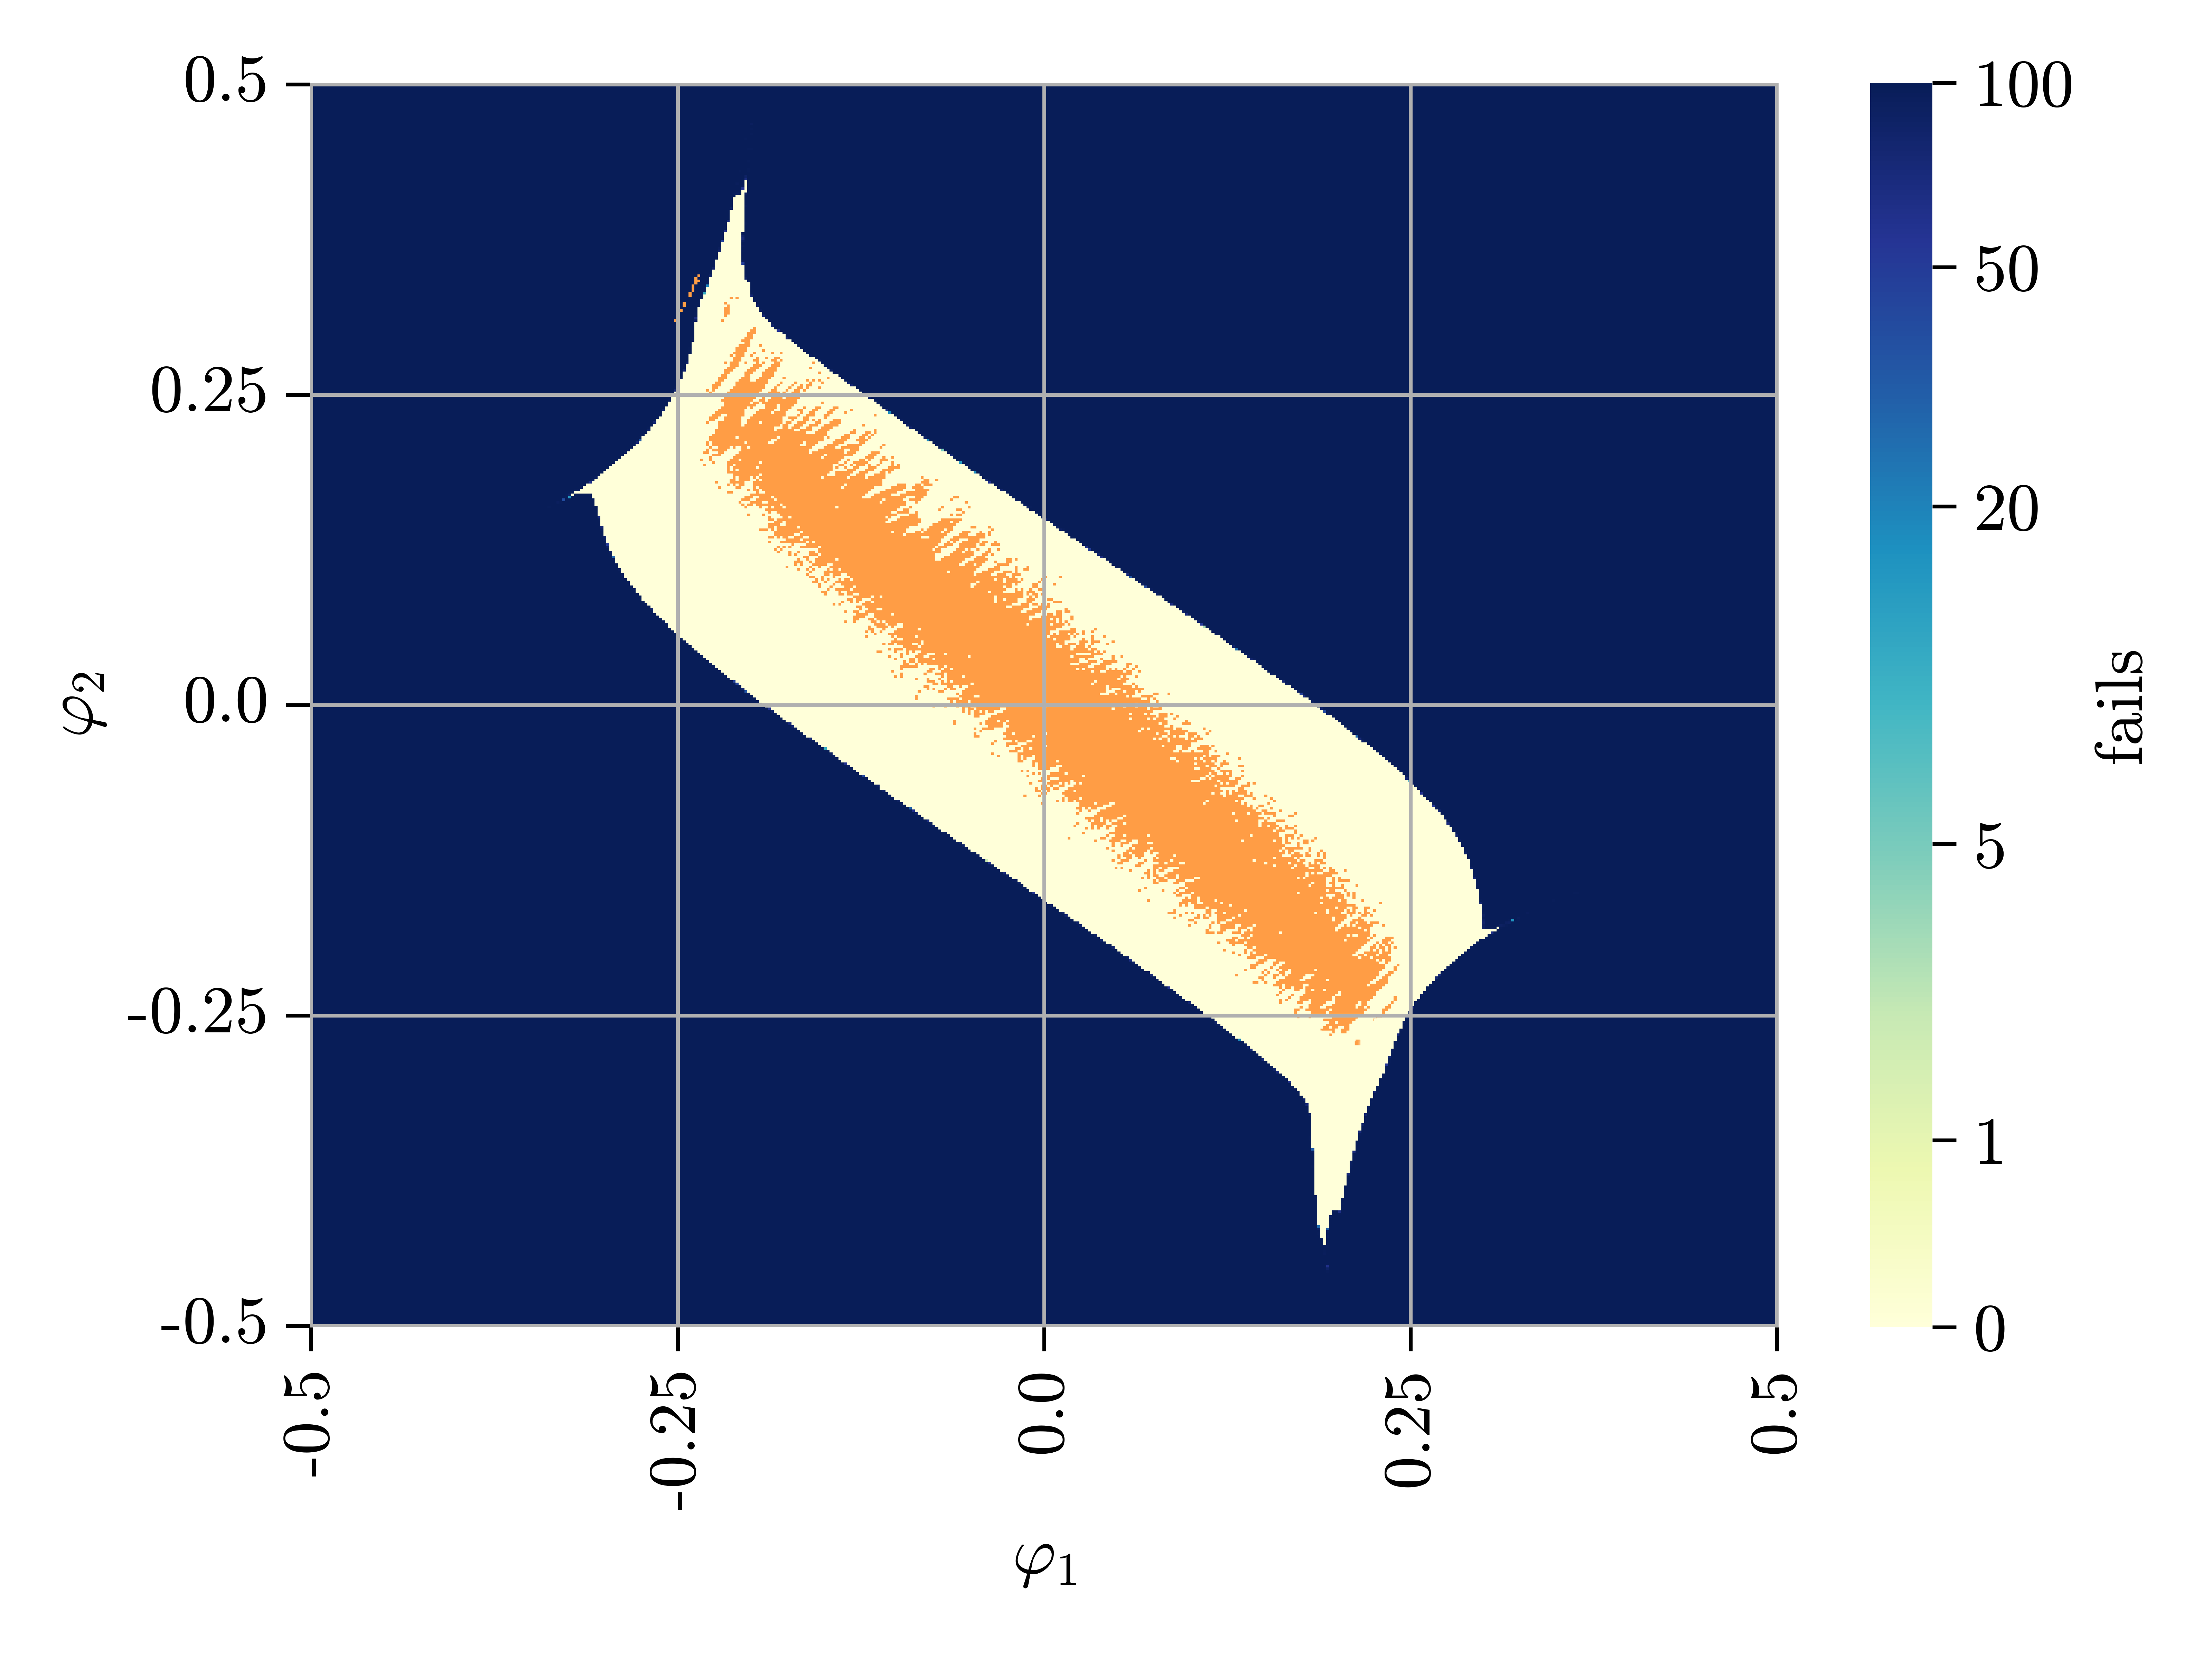
\includegraphics[width=\textwidth]{Figures/TP_continuous_vs_discrete_phi1phi2.png}
		\label{fig: tp - continuous vs discrete, phi1 phi2}
		\caption{}
	\end{subfigure}
	\hfill
	\begin{subfigure}[t]{0.48\textwidth}
		\centering
		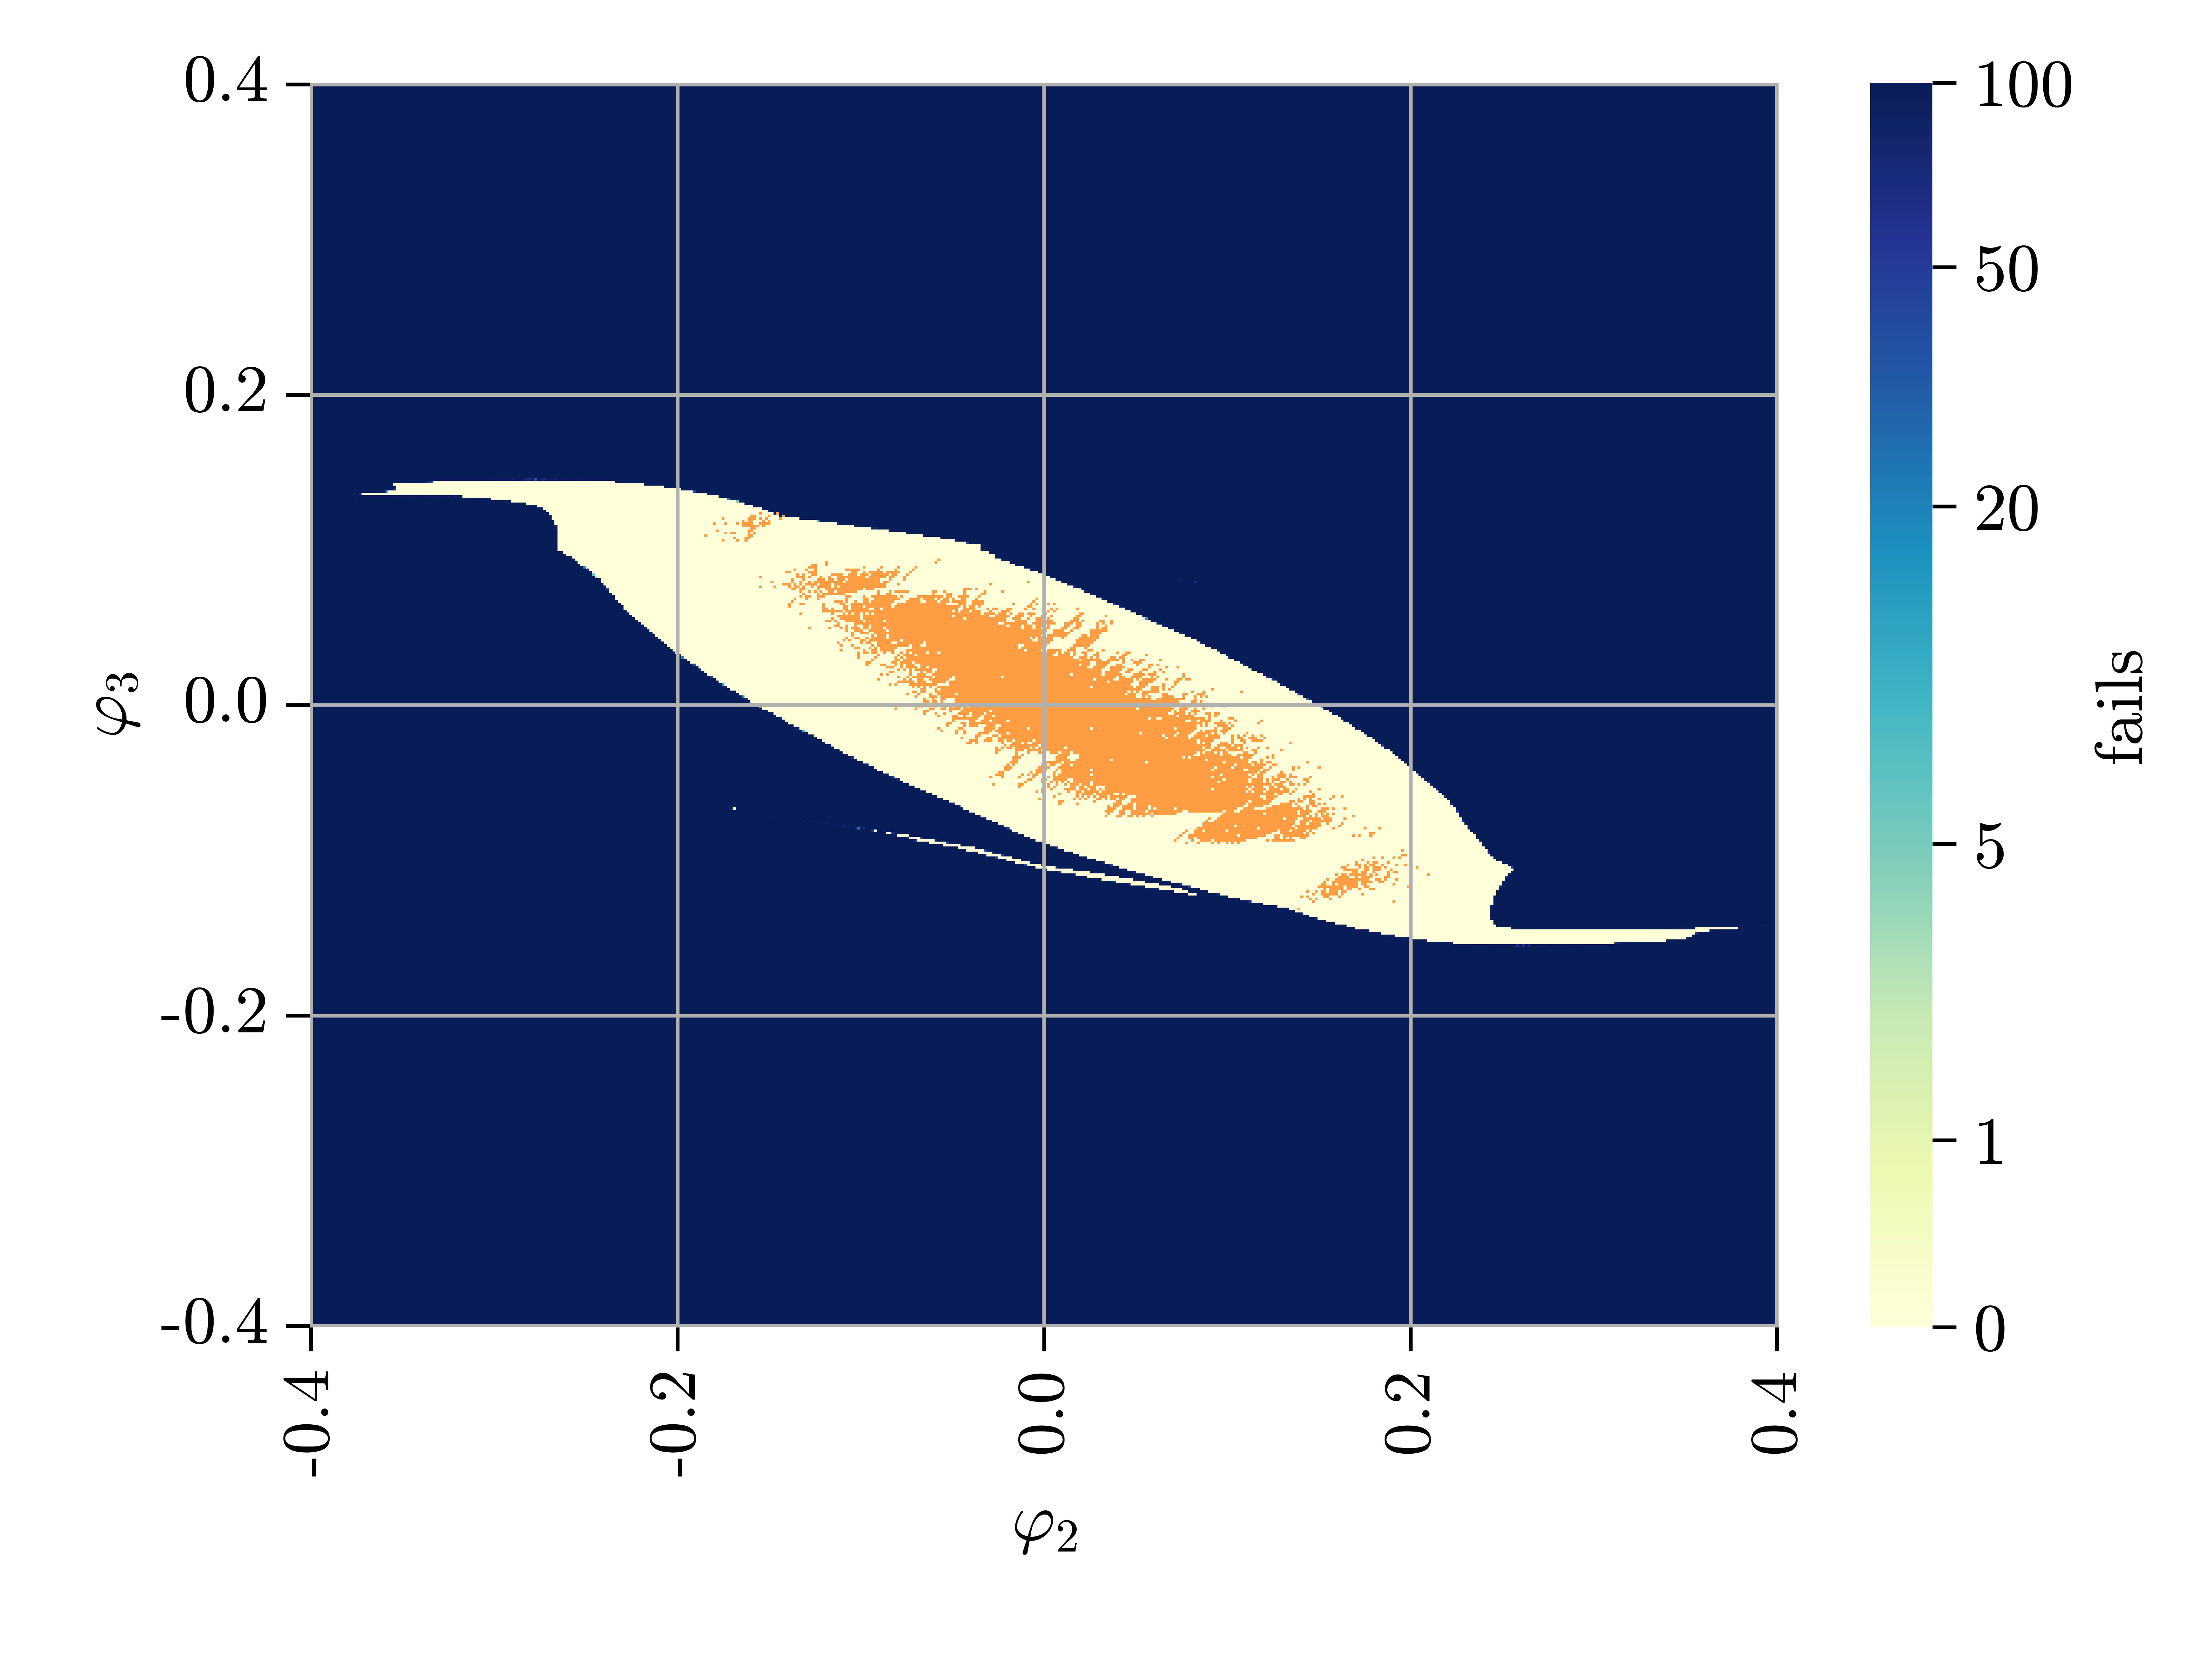
\includegraphics[width=\textwidth]{Figures/TP_continuous_vs_discrete_phi2phi3.png}
		\label{fig: tp - continuous vs discrete, phi2 phi3}
		\caption{}
	\end{subfigure}
	
	\caption{Stability zones comparison of the PPO agent using different control strategies. For the 1-link system (a) the zone axis are link's angle $\phi_1$ and angular velocity $\dot{\phi_1}$, while for the 2-link system (b) axis are the pendulum link angles $\phi_1$ and $\phi_2$. Figures (b) and (c) present the stability zones based on the dependence of pendulum link angles of $\phi_1$ and $\phi_2$ and of $\phi_2$ and $\phi_3$. The discrete control stability zone is indicated in orange; continuous is in white beige. Each grid cell represents 100 randomized tests.}
	\label{fig: continuous vs discrete}
\end{figure}

The training speed is also significantly different in terms of reaching the required amount of tests for the discrete and continuous control algorithm while it is not clearly seen for the 1- and 2-link systems.\todo{Unclear what you are saying. What is training speed? Where is the information about those tests that are required?} Comparison of it is shown at the Fig~\ref{fig: training time comparison}. To clarify what trains faster, the line, where the agent reaches maximum required amount of successful tests is drawn for each system with the shown time step. For all three cases the difference between the discrete and continuous control algorithm is around 45-50$\%$ in reaching the successful training, while for the triple pendulum the stable training using discrete control algorithm has be reached after 500 000 time steps.\todo{As above, you should refer to each subplot separately before providing general conclusions.}  

\begin{figure}[h!]
	\centering
	\begin{subfigure}[t]{0.48\textwidth}
		\centering
		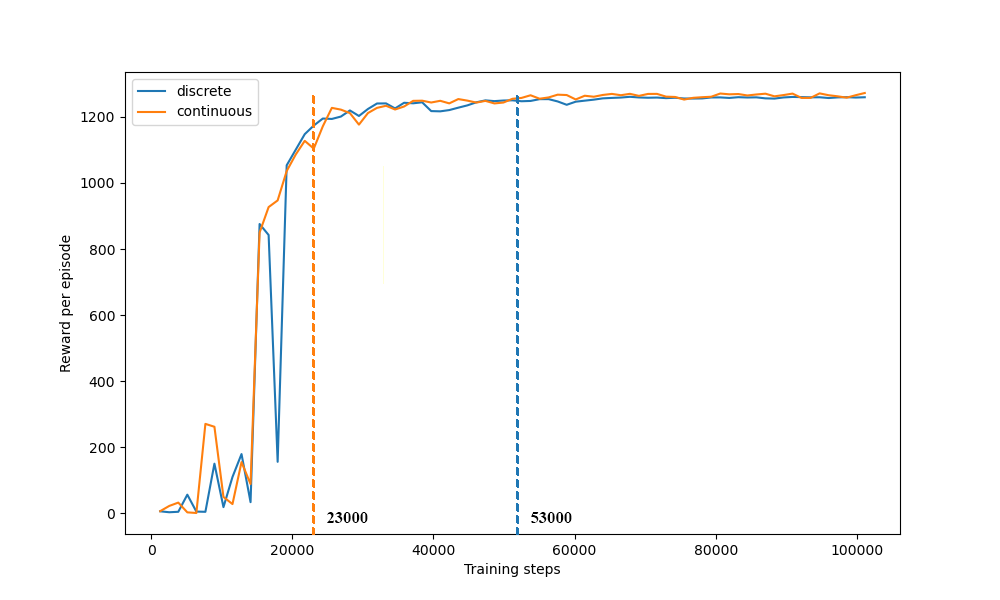
\includegraphics[width=\textwidth]{Figures/SP_discrete_vs_continuous_training_time.png}
		\label{fig: sp - training time}
		\caption{}
	\end{subfigure}
	\hfill
	\begin{subfigure}[t]{0.48\textwidth}
		\centering
		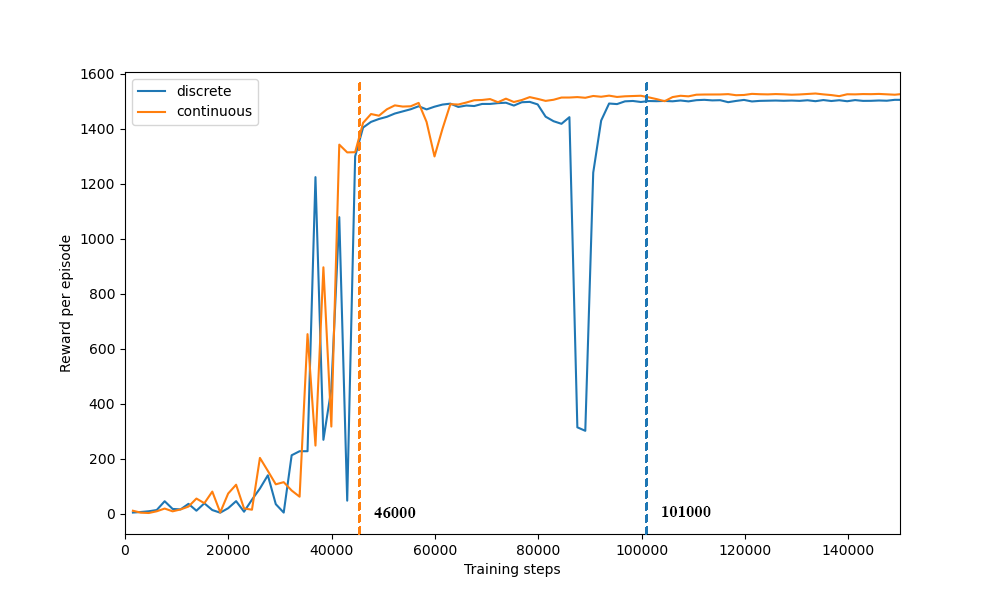
\includegraphics[width=\textwidth]{Figures/DP_discrete_vs_continuous_training_time.png}
		\label{fig: dp - training time}
		\caption{}
	\end{subfigure}
	\begin{subfigure}[t]{0.48\textwidth}
		\centering
		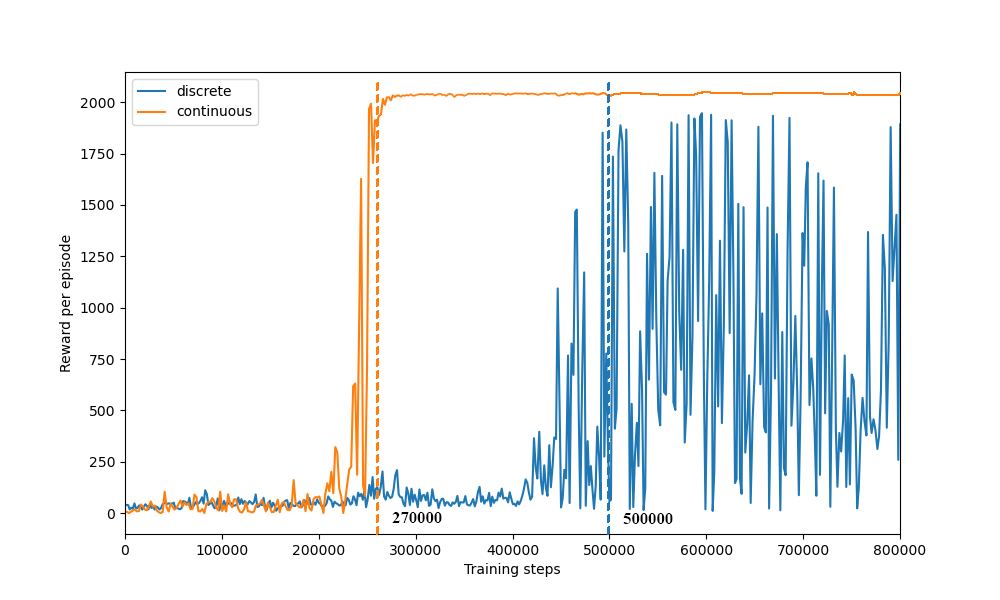
\includegraphics[width=\textwidth]{Figures/TP_discrete_vs_continuous_training_time.png}
		\label{fig: tp - training time}
		\caption{}
	\end{subfigure}
	
	\caption{Training times for the PPO agents for 1-link (a), 2-link (b) and 3-link (c) systems}
	\label{fig: training time comparison}
\end{figure}

Our results show, that not even the operating area of the RL agent is wider and smoother, but the agent also achieves a faster training result. 

\subsection{Agents with continous action space tested on modified environments} \label{subsec: Agent tested on modified environments}

In this section, we examine the impact of changing properties of the environment, namely
link length, mass, and added friction, on the stability zones.\todo{Provide more details, refer actual parameters, what friction, where, refer to Figures, etc.} The investigation is conducted
using the inverted double pendulum on a cart model (same continuous agent as in the Figure~\ref{fig: continuous vs discrete} (b)). In each subplot of Figure~\ref{fig: agent impact on different environments}, the stability zone is determined for the same agent in various modified environments, and the contour of the stability zone from the original environment is overlaid. Friction is implemented using the same method as in our previous research~\cite{manzl2023relrl}.\todo{Provide details here as this should not take long to describe it.}

 \begin{figure}[h!]
     \centering
     \begin{subfigure}[t]{0.32\textwidth}
         \centering
         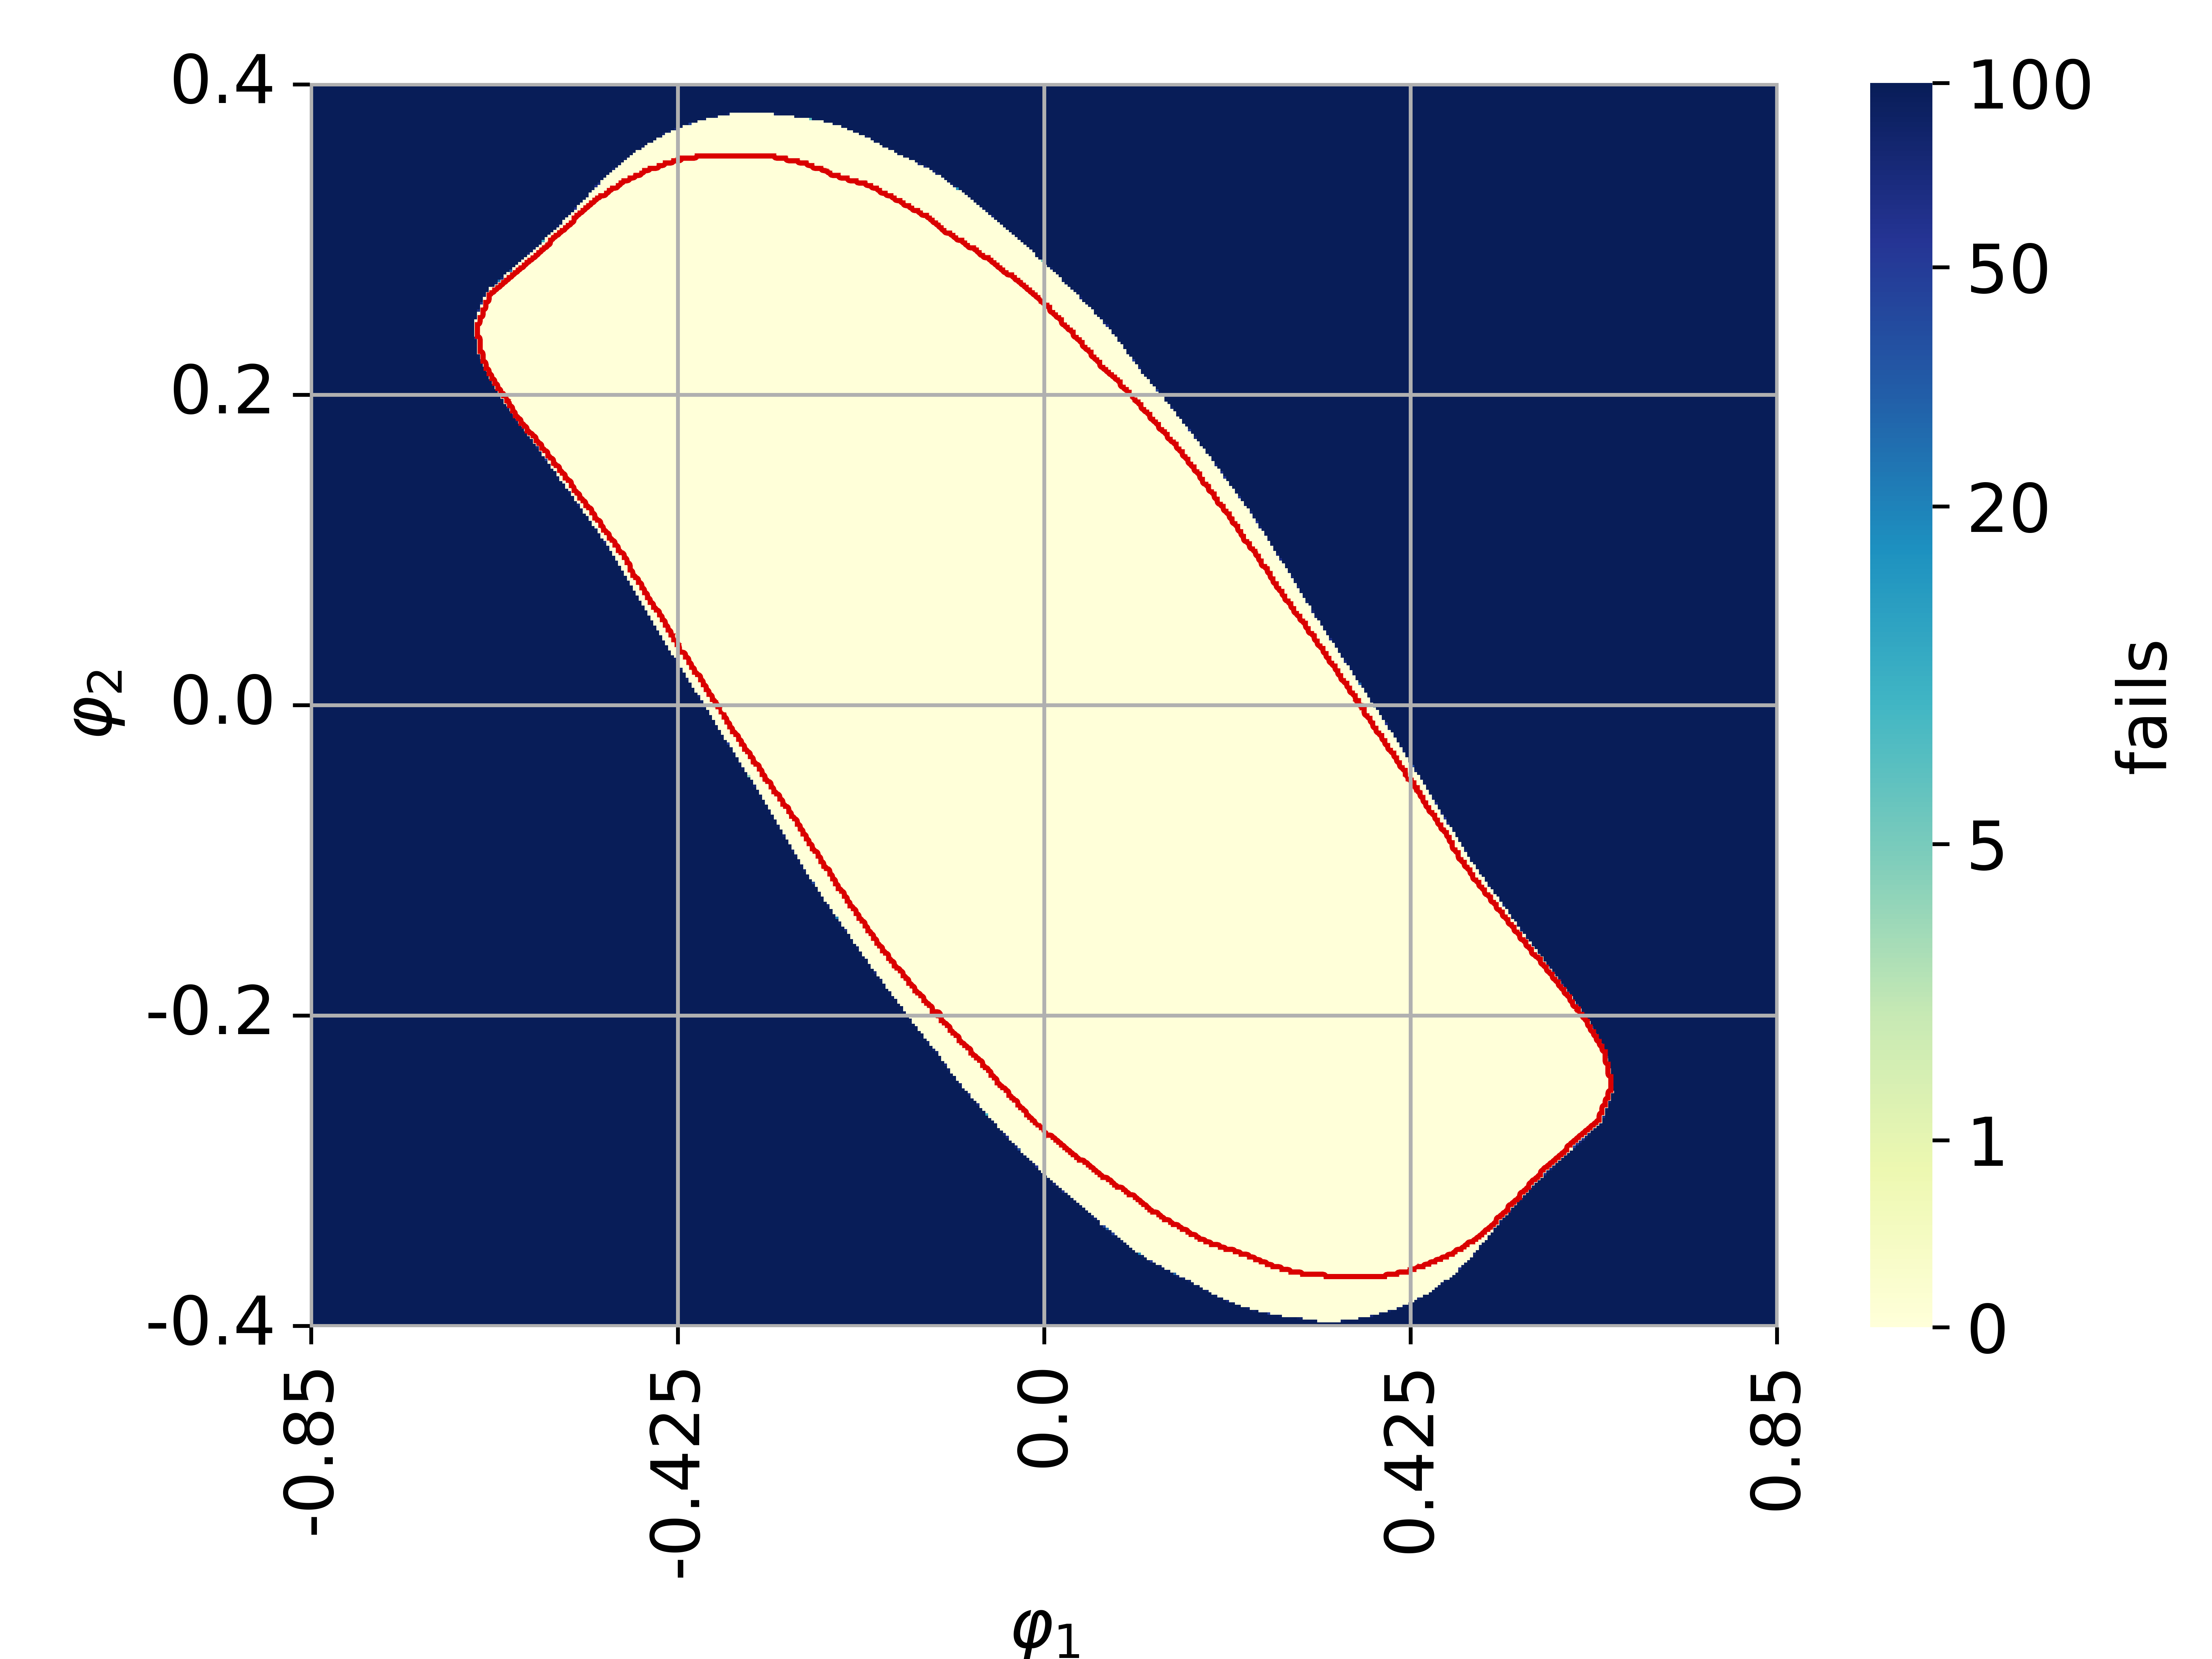
\includegraphics[width=\textwidth]{Figures/DP_len_1.1.png}
         \label{fig: DP len 1.1}
         \caption{}
     \end{subfigure}
     \hfill
     \begin{subfigure}[t]{0.32\textwidth}
         \centering
         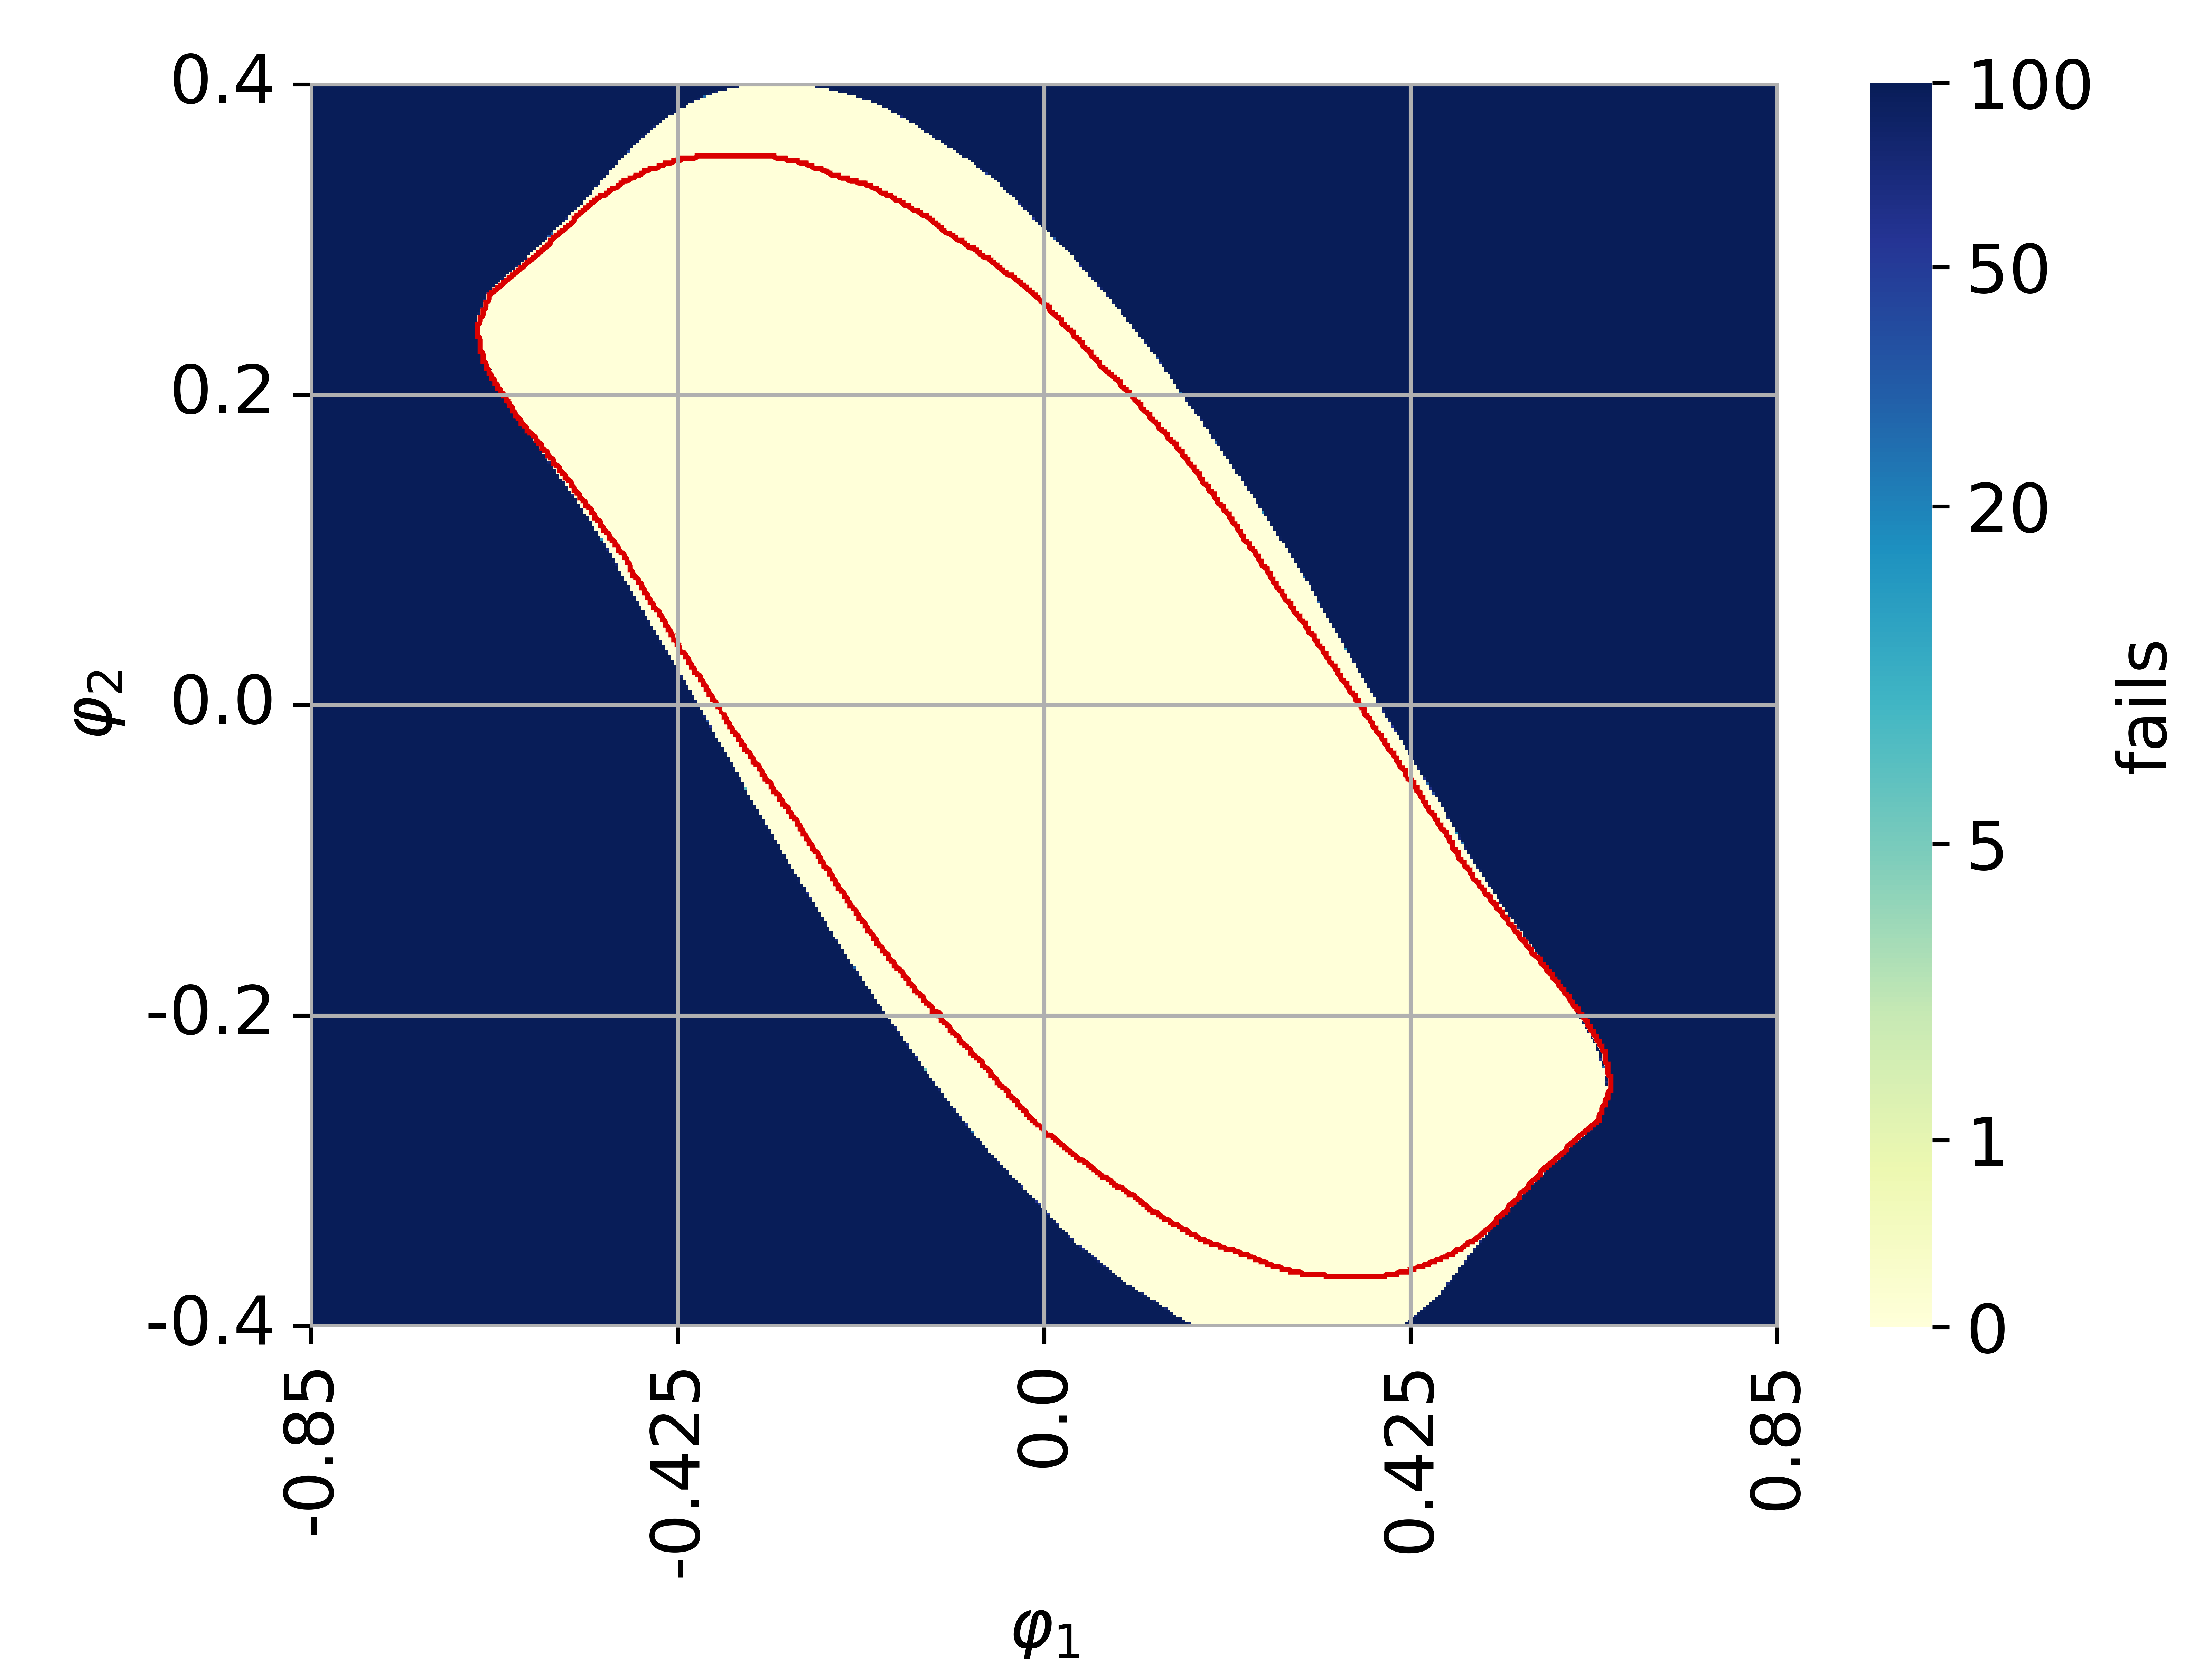
\includegraphics[width=\textwidth]{Figures/DP_len_1.2.png}
         \label{fig: DP len 1.2}
         \caption{}
     \end{subfigure}
     \hfill
     \begin{subfigure}[t]{0.32\textwidth}
         \centering
         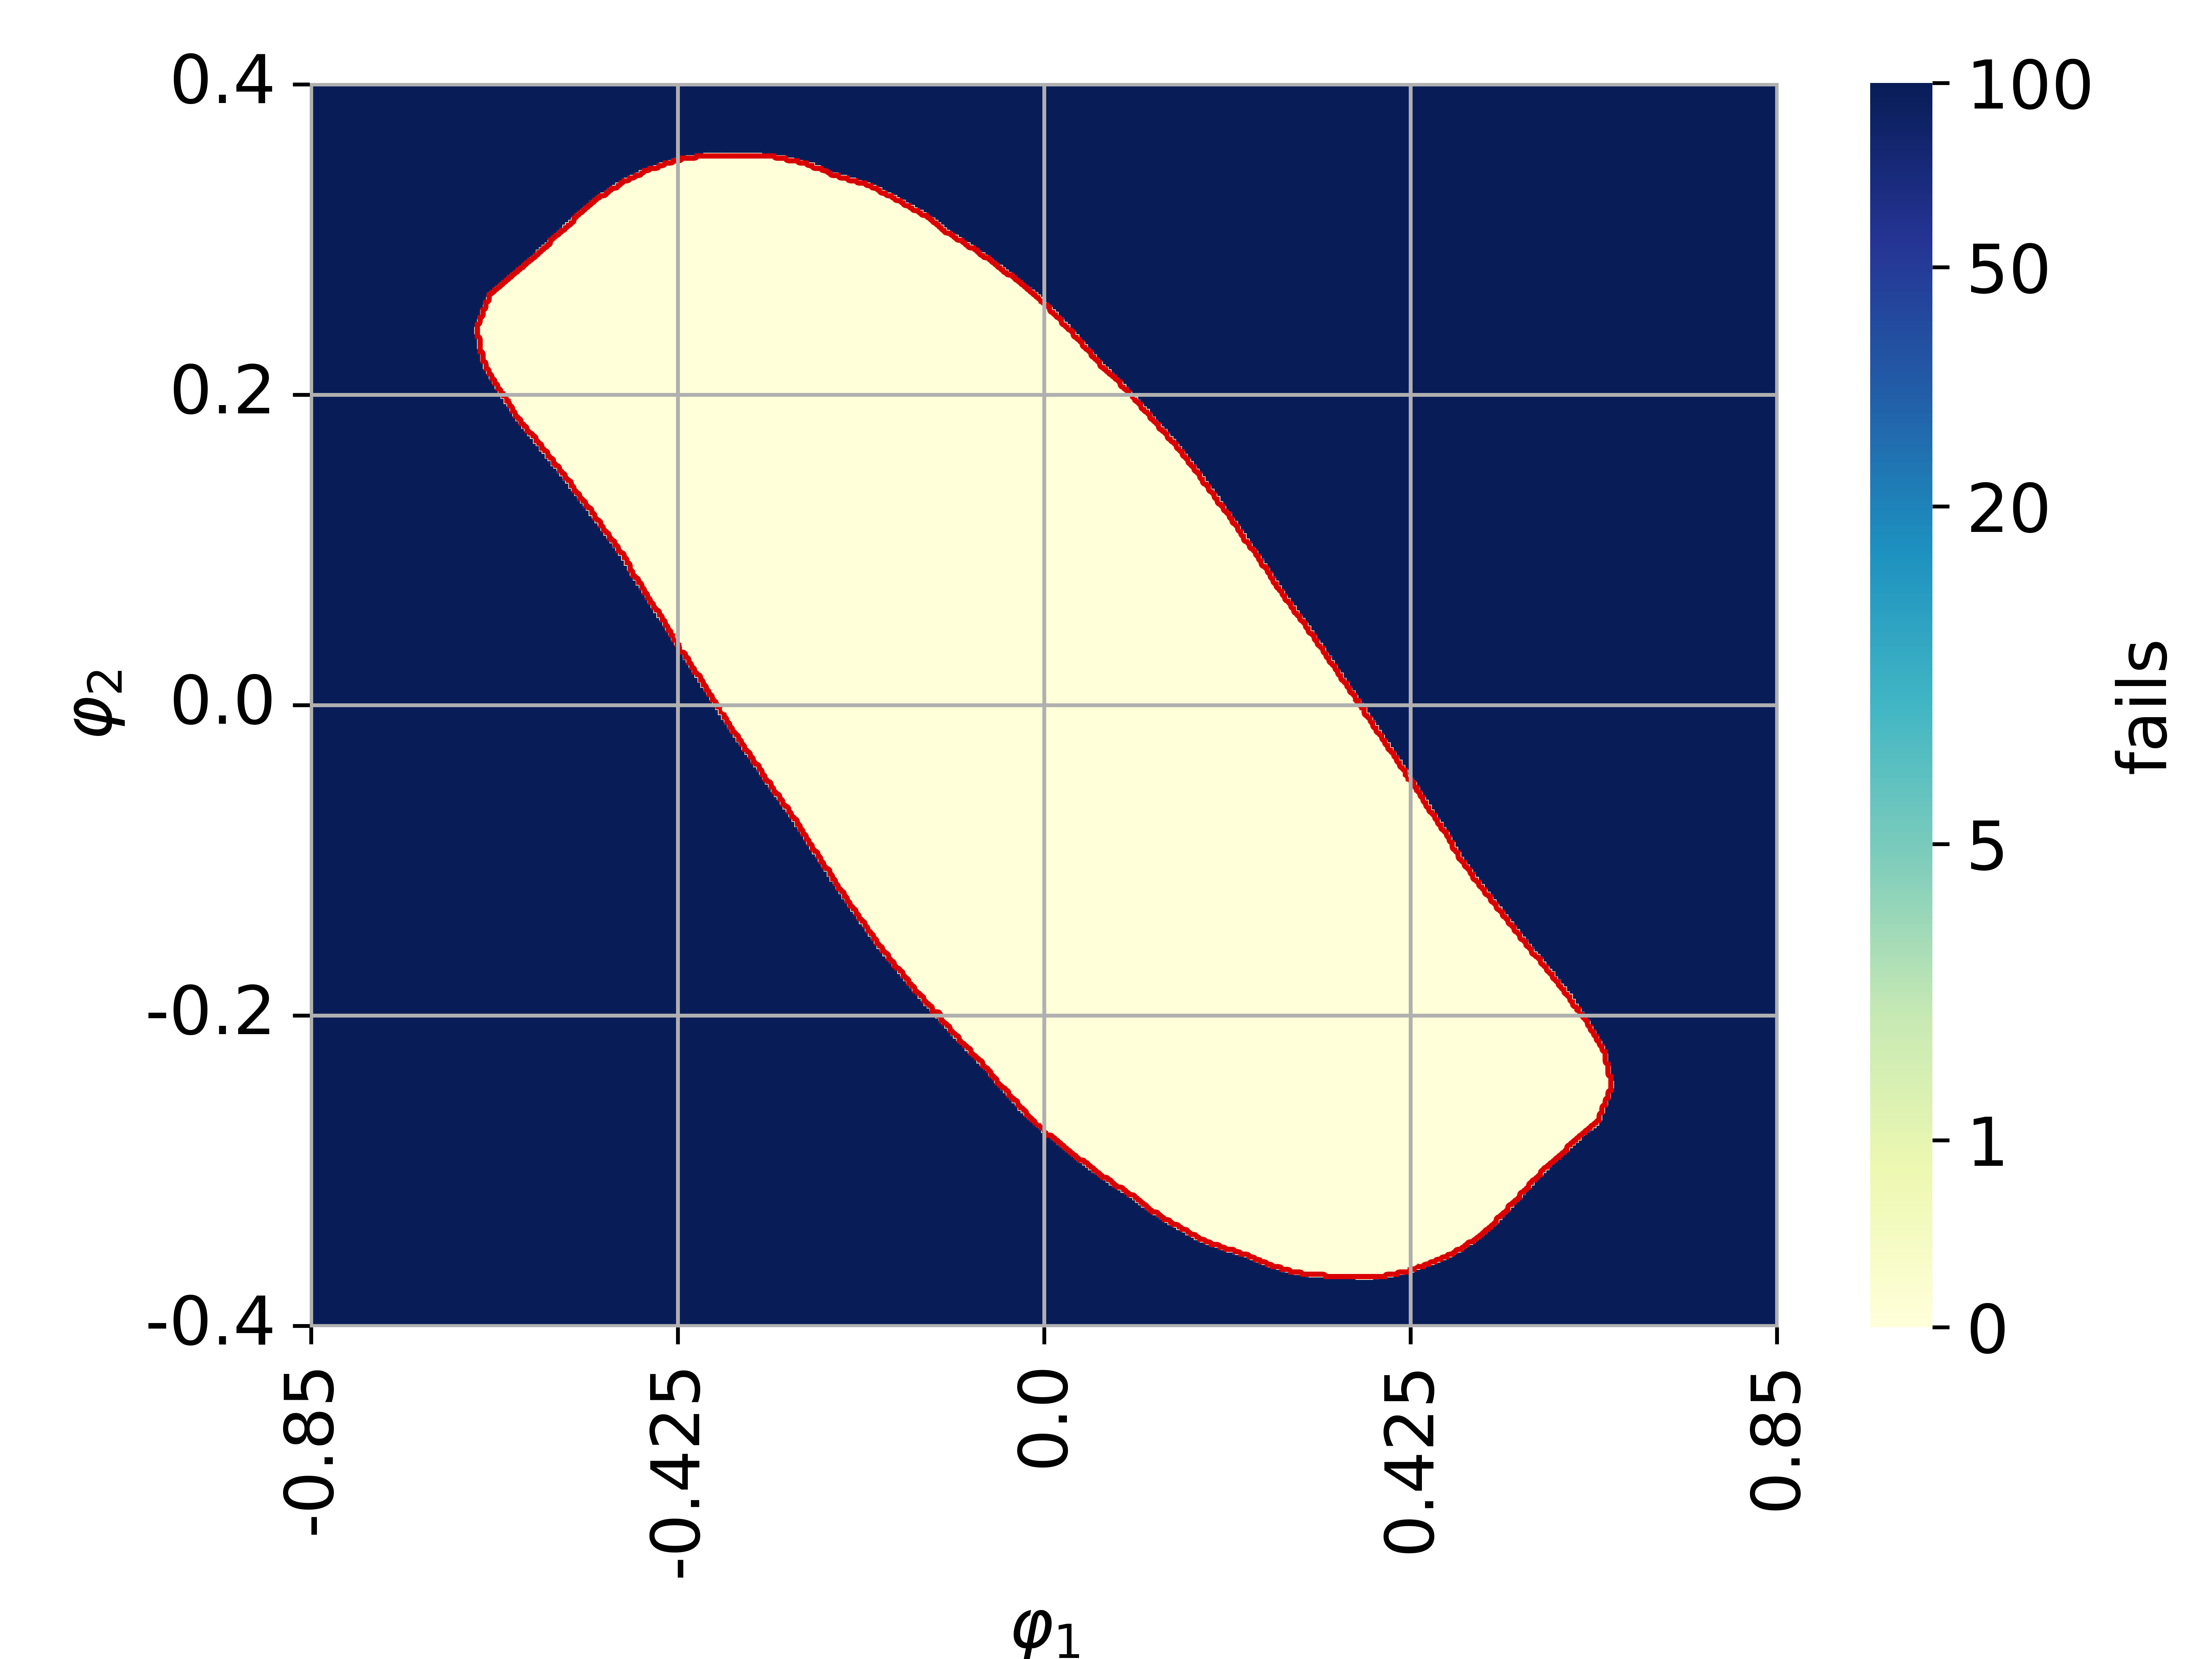
\includegraphics[width=\textwidth]{Figures/DP_mass_1.1.png}
         \label{fig: DP mass 1.1}
         \caption{}
     \end{subfigure}

     \vspace{0.2cm}

     \begin{subfigure}[t]{0.32\textwidth}
         \centering
         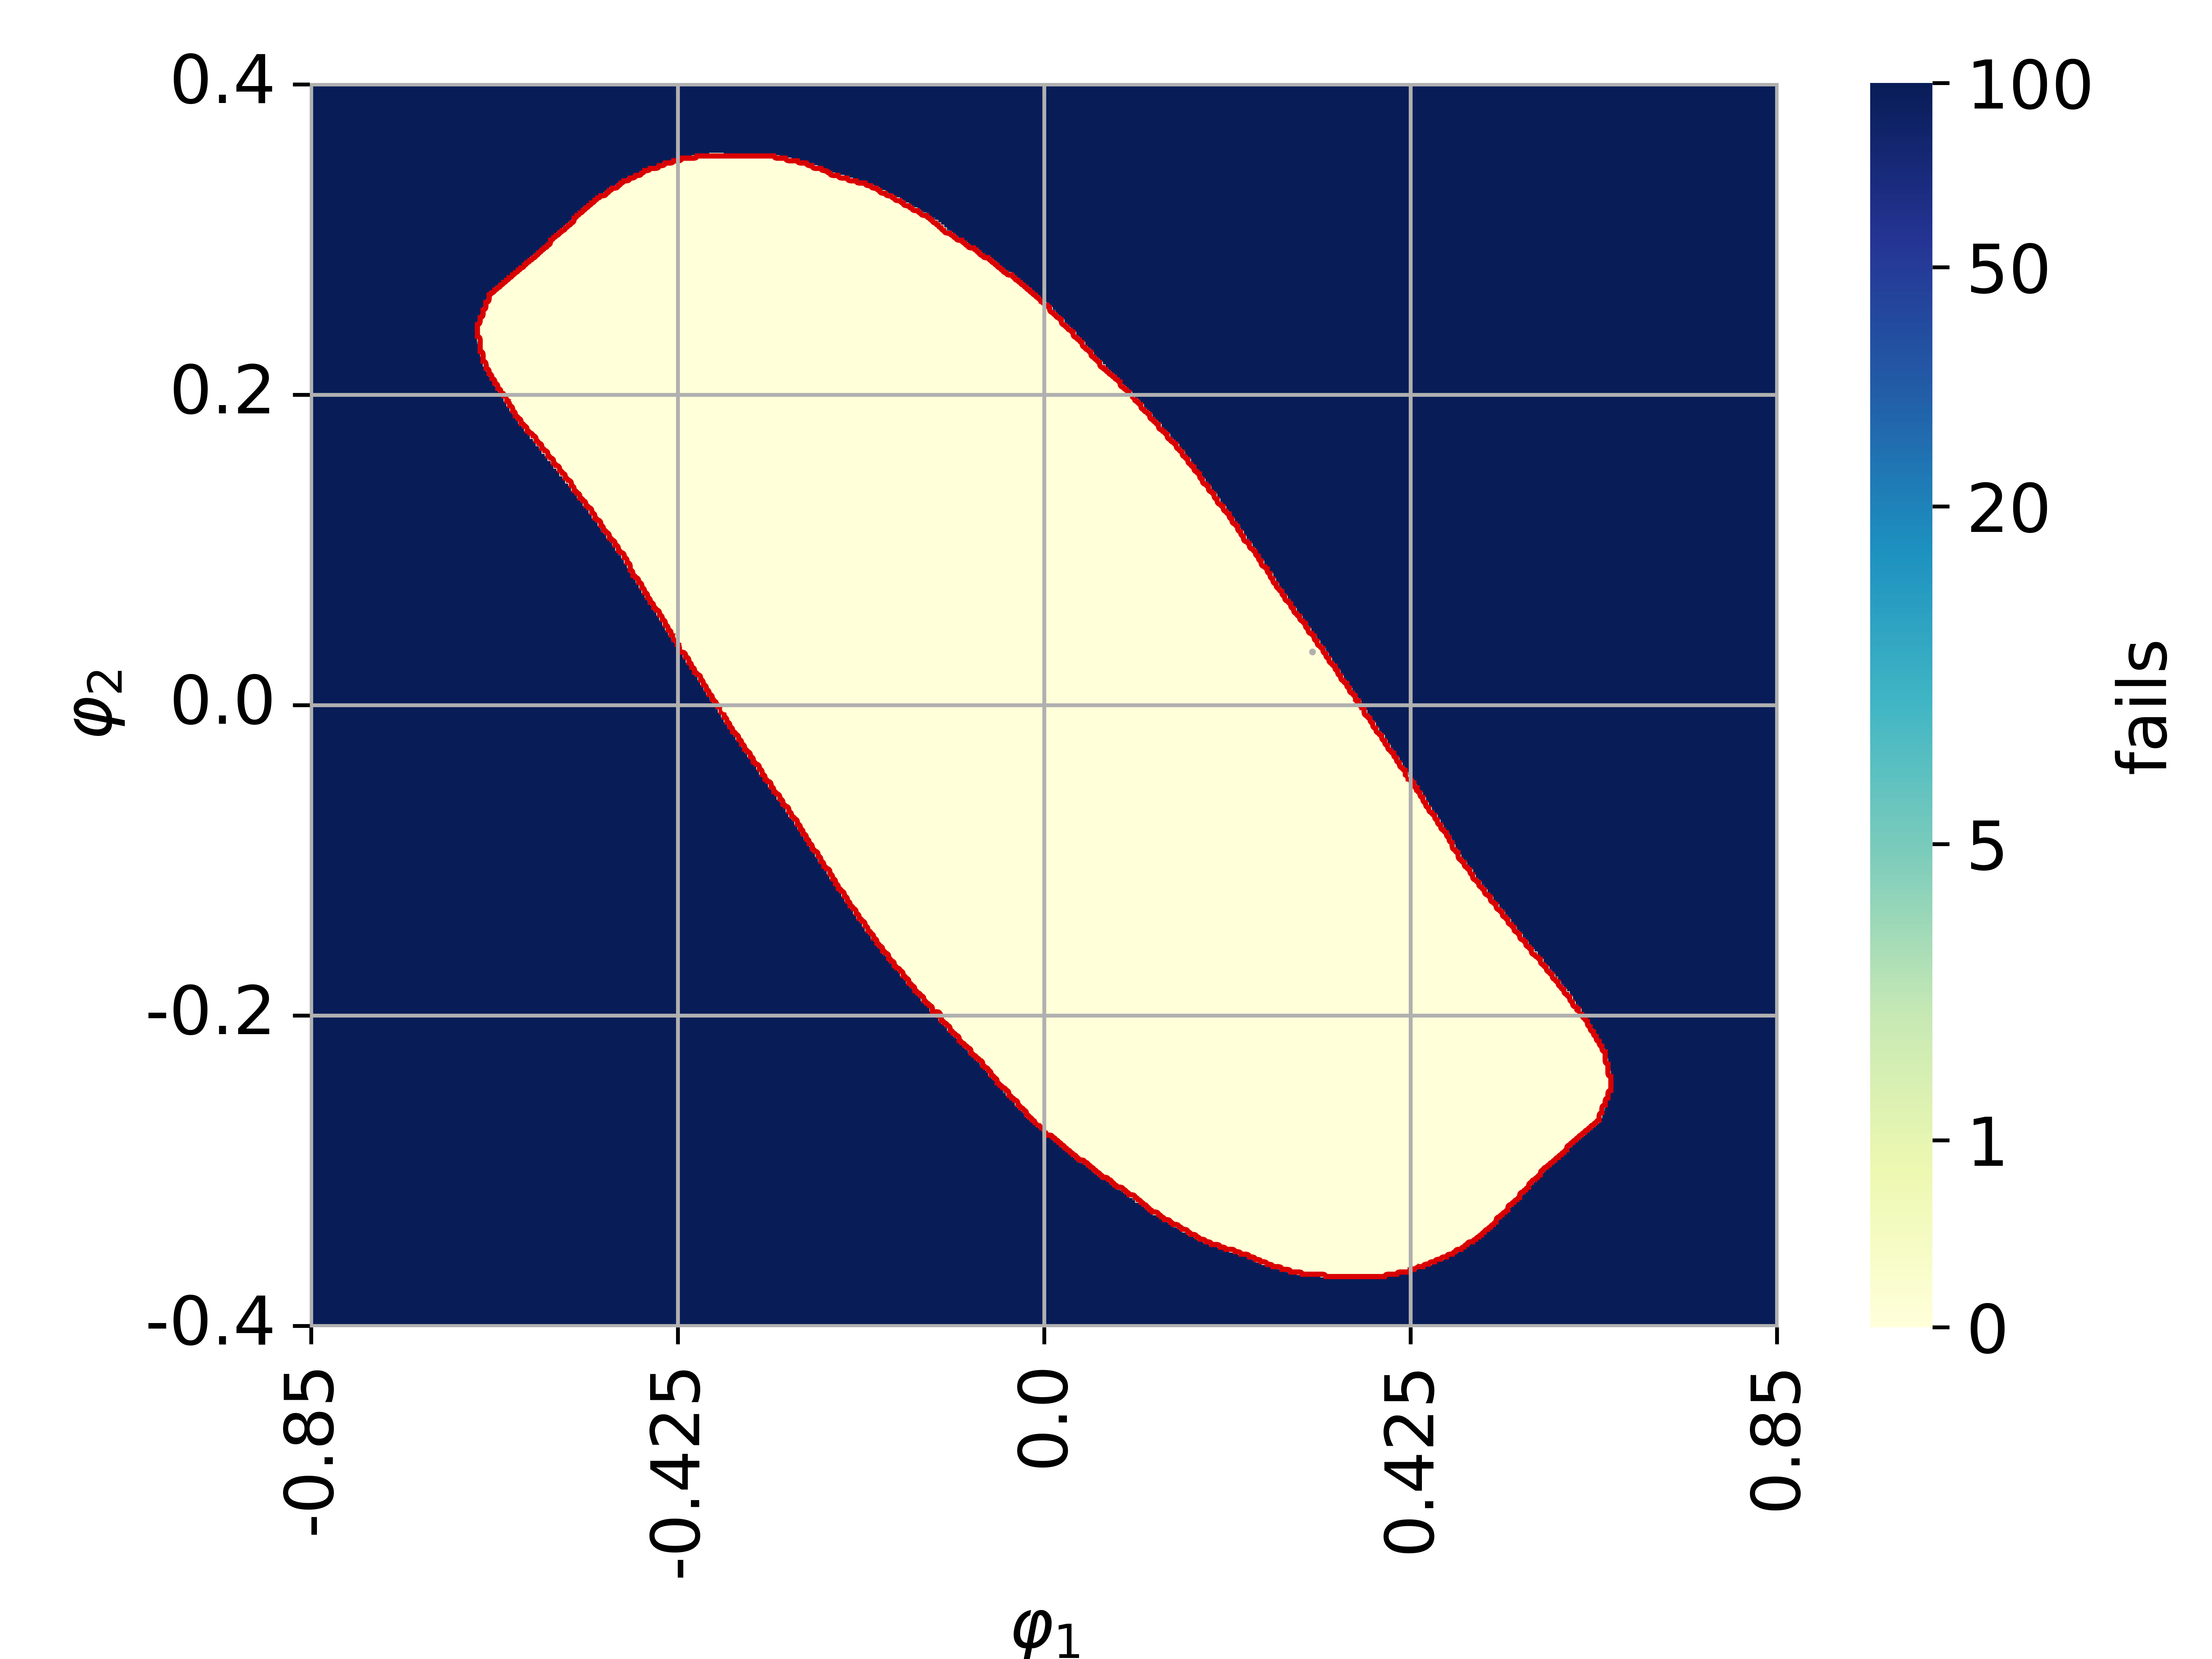
\includegraphics[width=\textwidth]{Figures/DP_mass_1.2.png}
         \label{fig: DP mass 1.2}
         \caption{}
     \end{subfigure}
     \hfill
     \begin{subfigure}[t]{0.32\textwidth}
         \centering
         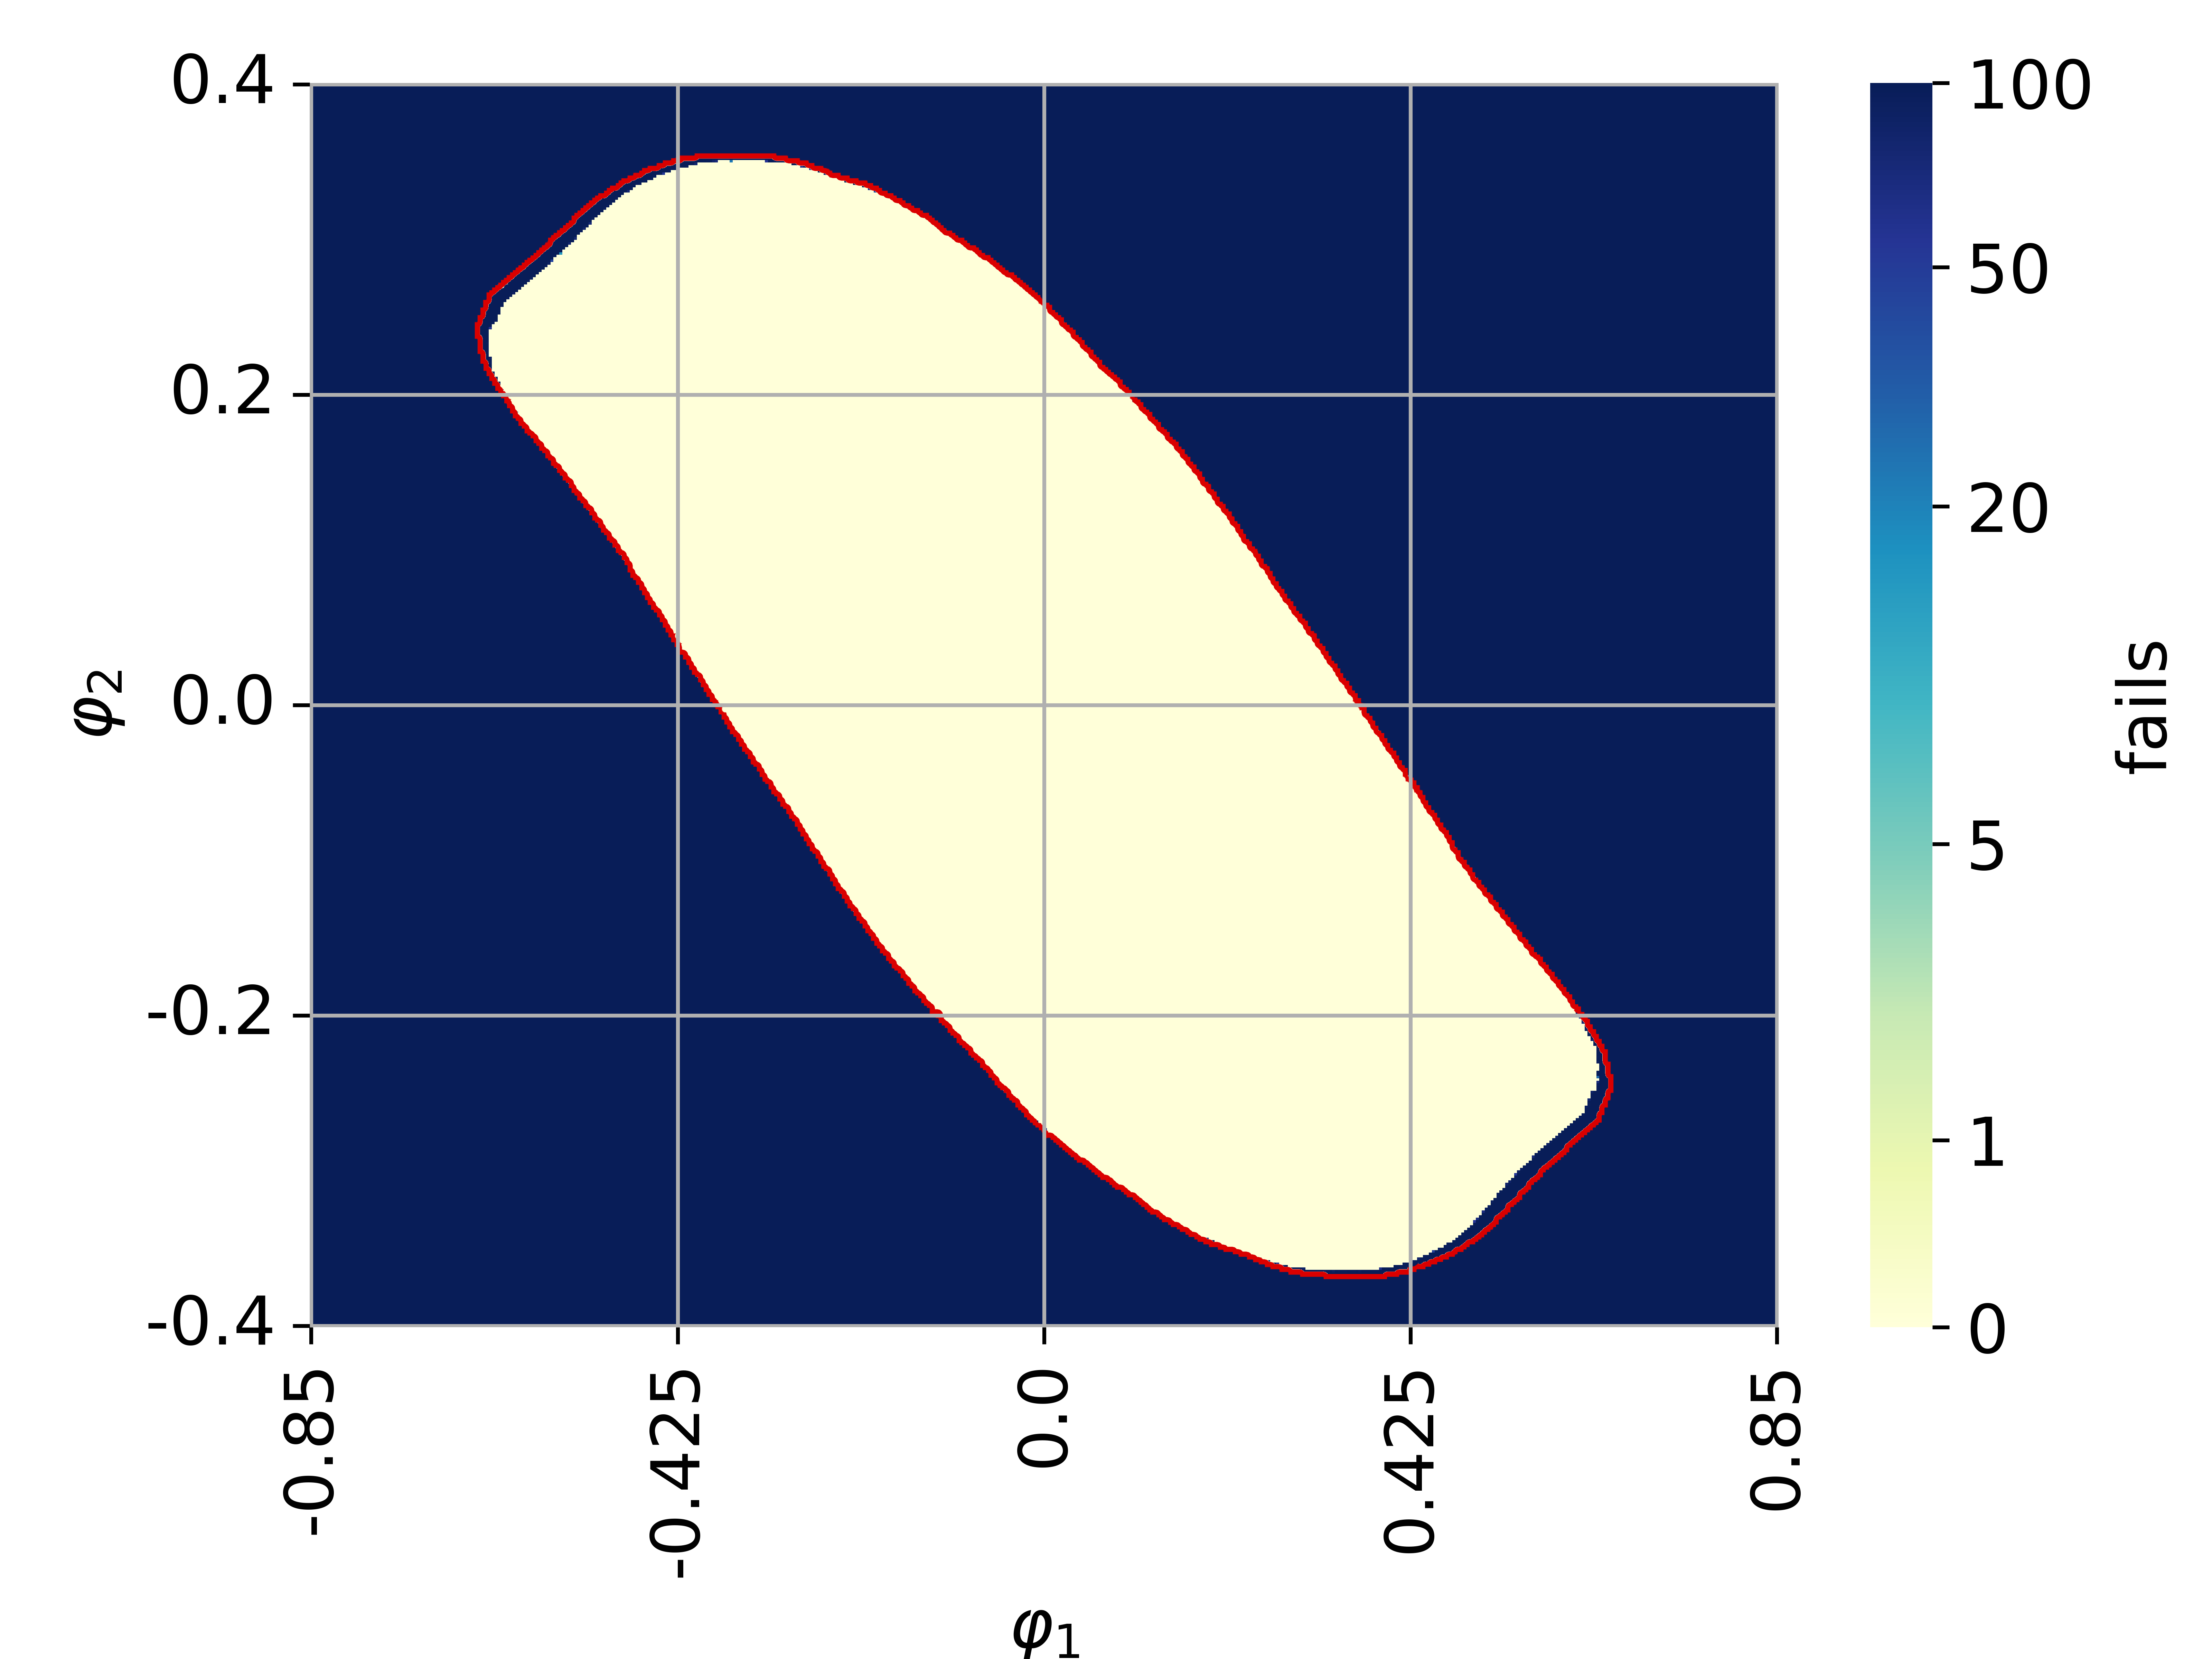
\includegraphics[width=\textwidth]{Figures/DP_friction_0.01.png}
         \label{fig: DP friction 0.01}
         \caption{}
     \end{subfigure}
     \hfill
     \begin{subfigure}[t]{0.32\textwidth}
         \centering
         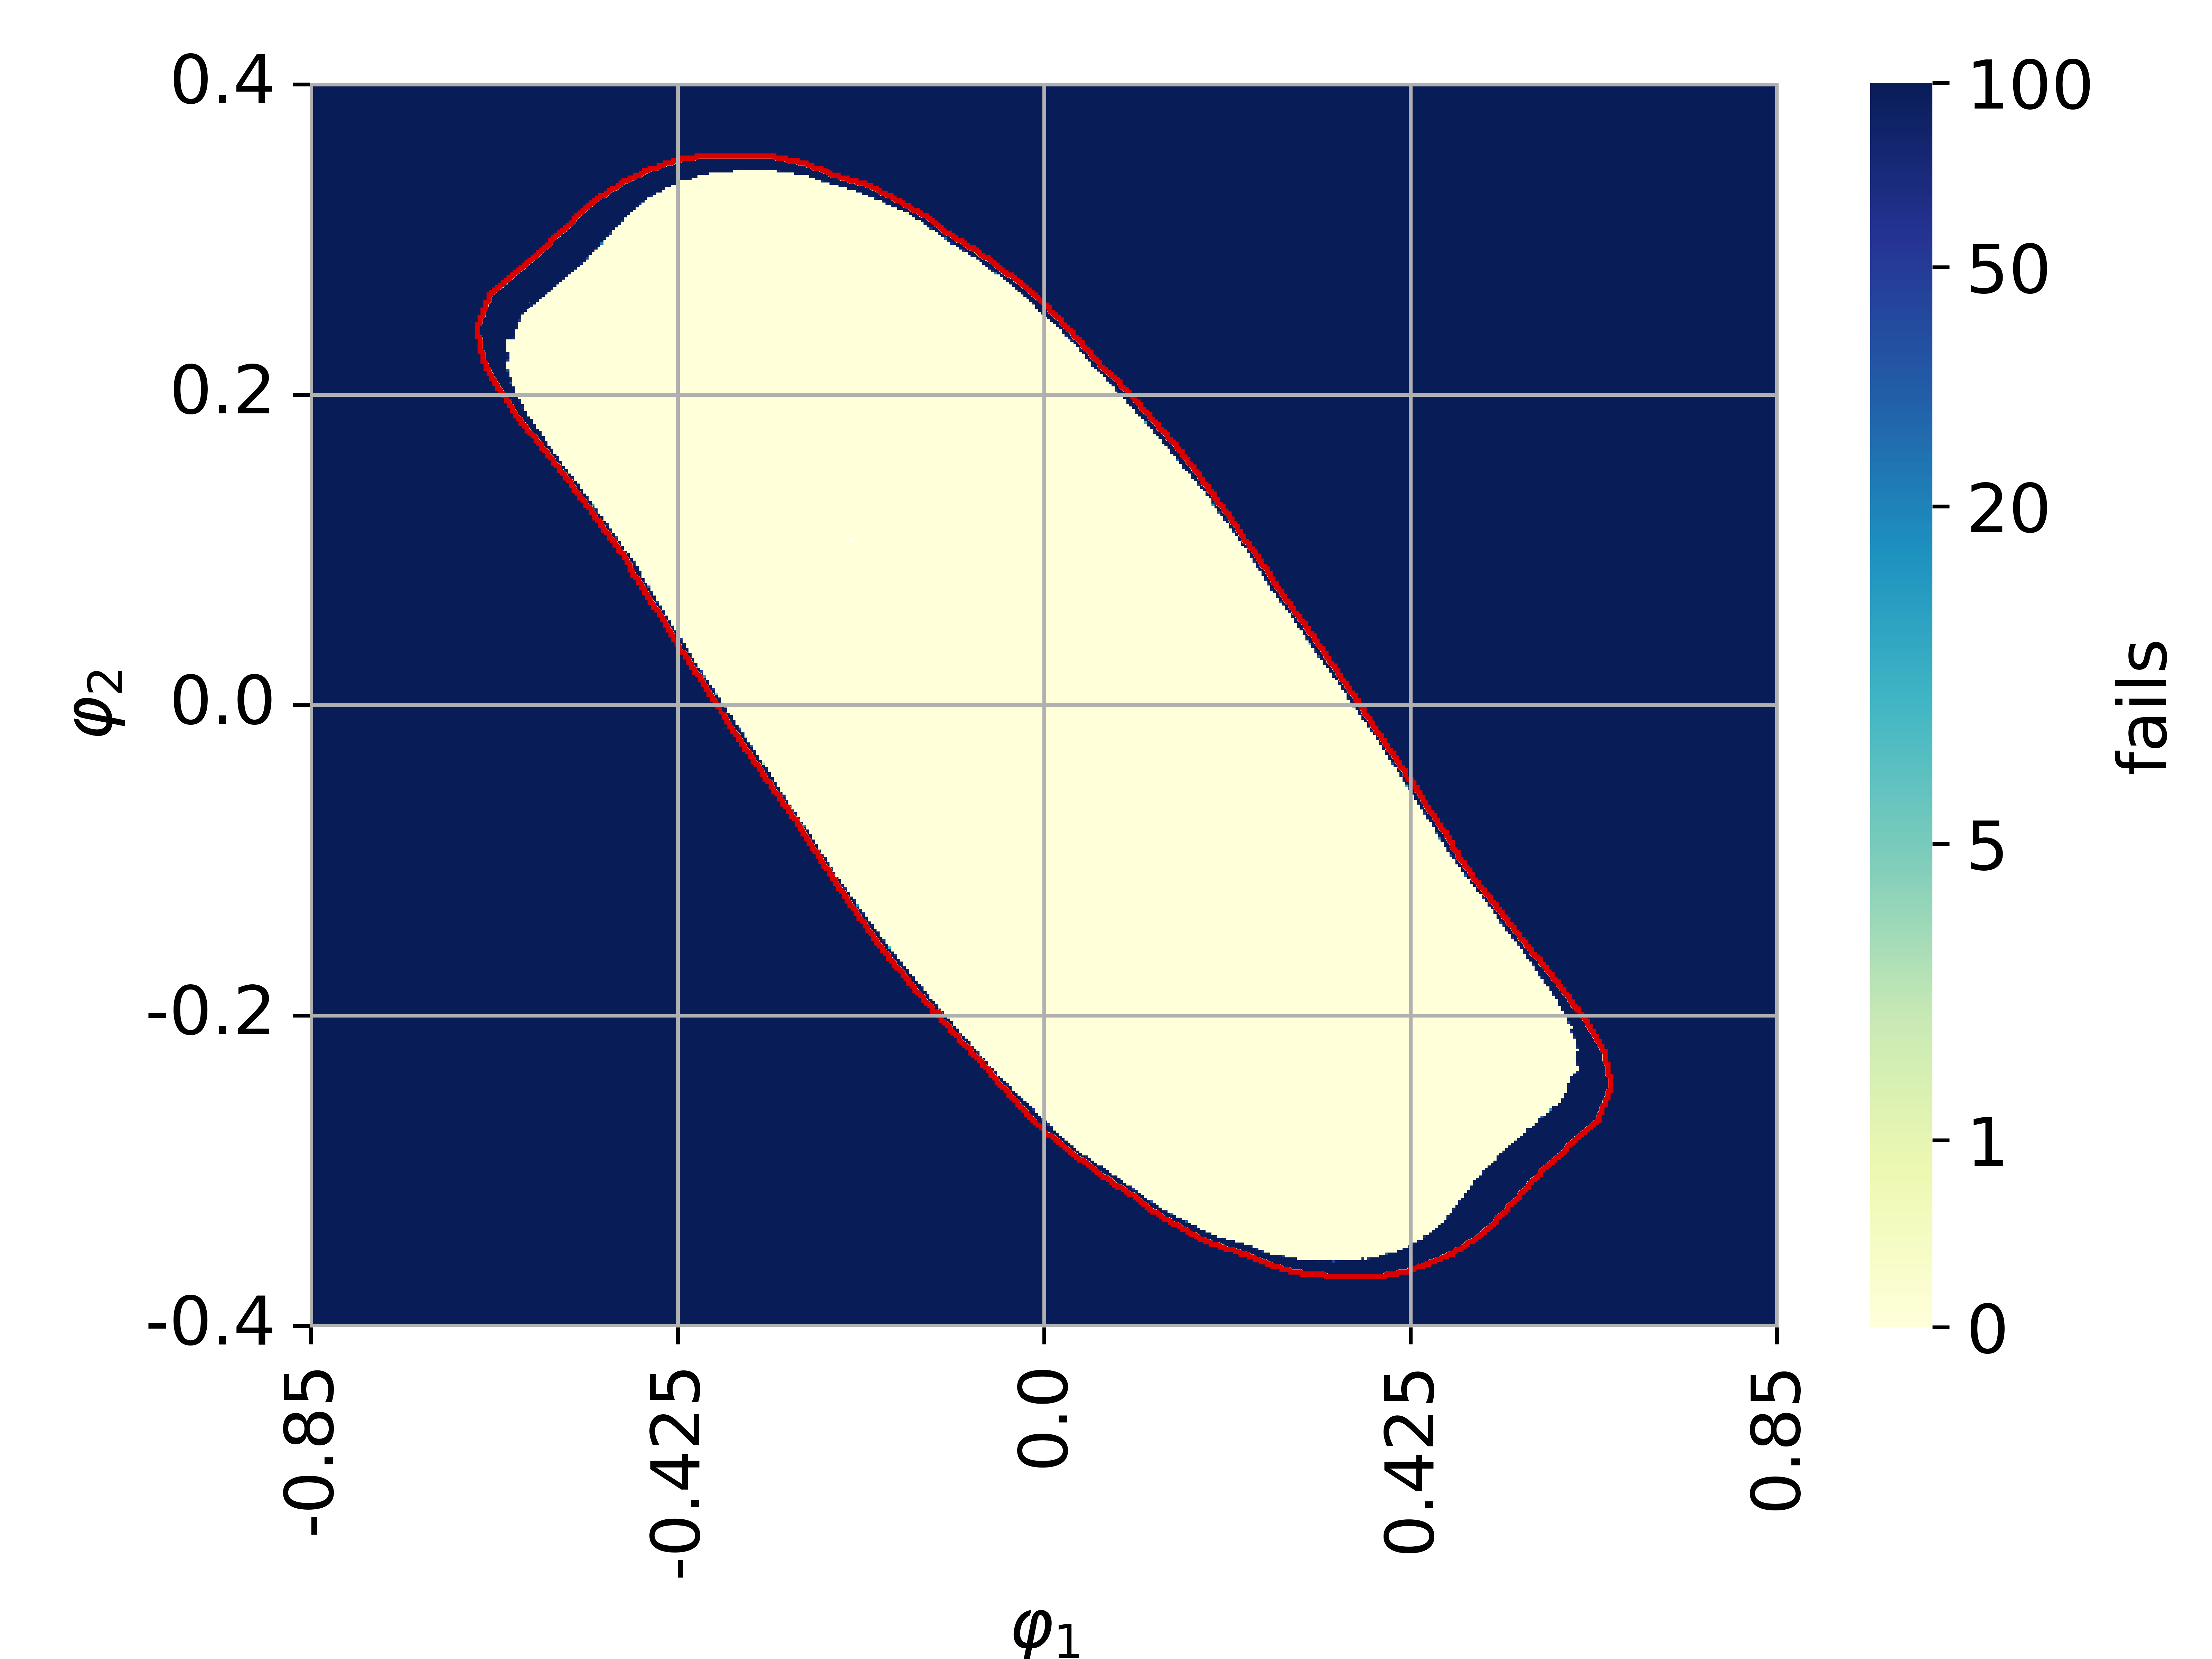
\includegraphics[width=\textwidth]{Figures/DP_friction_0.02.png}
         \label{fig: DP friction 0.02}
         \caption{}
     \end{subfigure}

     \caption{The stability zone for the double link system using the PPO agent, case 0. The red boundary corresponds to that depicted continuous control stability zone in Figure~\ref{fig: continuous vs discrete} (b). The environment parameters are modified as follows: (a) 1.1~$l$, (b) 1.2~$l$, (c) 1.1~$m$, (d) 1.2~$m$, (e) $f_rel$ = 0.01, and (f) $f_rel$ = 0.02.}
     \label{fig: agent impact on different environments}
 \end{figure}

The observations shows, that increasing the link length will cause the stability zone to expand, while not having the increase of the blind spots, as it was for the discrete control cases~\cite{manzl2023relrl}.\todo{Refer to the figures. It seems that the longer the link, the larger is the change. Consider testing what happens when link is shorten. More details about behavior of the system in the original work. Does it also increases? By same factor?} Increasing the mass of the link doesn't provide any differences from the base model, so that we can state that up to the changes of 20$\%$ the model is independent from the link mass change.\todo{How it was for discrete? The same?}
Considering friction the stability zone becomes smaller within each increase of it, but the value of \( f_{\text{rel}} = 0.02 \) still provides us with the stable zone without causing the agent to fail in the original contour, as it was shown in~\cite{manzl2023relrl}. It can be concluded that the continuous control scheme is more suitable if friction is involved in the environment model simulation.

\subsection{RL training enhancement with CL} \label{subsec: RL training enhancement with CL}
To select the parameters needed for the CL implementation the research was conducted in the following fashion. At first, we determine which decay type is specifically the most performing for our particular task of pendulum stabilization. For this we have simulated 150 runs of 5 cases within the control values matrix of the form 
\(\begin{bmatrix} 1 & n \\ 0 & 0 \end{bmatrix}\), where \(n = 2, 4, 6, 8, 10\) and decay steps vector \(\begin{bmatrix} 0 \\ k \end{bmatrix}\), where \(k = 5000, 6000, \ldots, 10000\) to evaluate the performance across different control parameters. The results are presented in a form of a bar plot, which shows the number of agent successes for the whole dataset. It is shown, that the exponential decay type function, provides the best results of having 74$\%$ of successes across the dataset. Within this research conducted, in the next steps we have used this decay type to work with for the CL implementation. 

\begin{figure}[h]
	\centering
	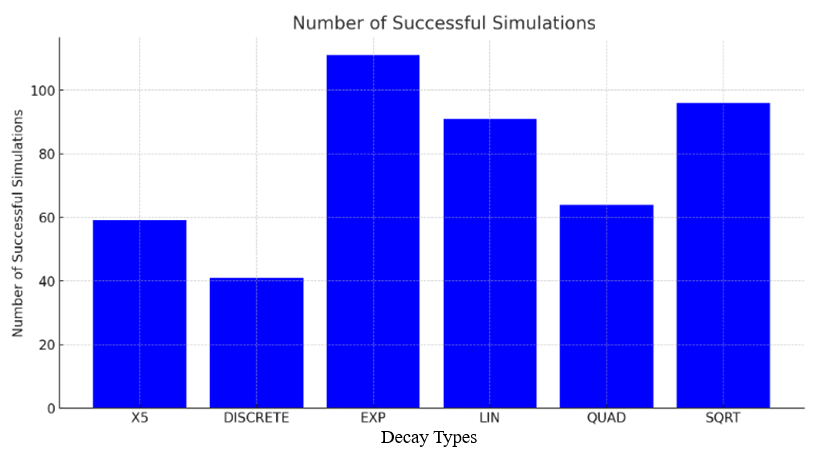
\includegraphics[width=10cm]{Figures/decay_types_results_comparison.png}
	\caption{}
	\label{fig: decay types comparison}
\end{figure}


\section{Conclusions}




\printbibliography

\end{document}
